% =====================================================================
%  Documentazione tecnica del progetto
%  "Sistema di pianificazione degli appelli"
%  Monorepo Nx full-stack: NestJS (API) + React (UI) + PostgreSQL
% =====================================================================
\documentclass[11pt,a4paper,oneside]{report}

% ---- Codifica e lingua --------------------------------------------------
\usepackage[utf8]{inputenc}
\usepackage[T1]{fontenc}
\usepackage[italian]{babel}
\usepackage{lmodern}
\usepackage{microtype}

% ---- Layout e grafica ---------------------------------------------------
\usepackage[a4paper,margin=2.6cm]{geometry}
\usepackage{graphicx}
\usepackage{xcolor}
\usepackage{tikz}
\usetikzlibrary{shapes.geometric,arrows.meta,positioning,fit,backgrounds,calc}
\usepackage{booktabs}
\usepackage{tabularx}
\usepackage{array}
\usepackage{longtable}
\usepackage{enumitem}
\usepackage{fancyhdr}
\usepackage{titlesec}

% ---- Codice -------------------------------------------------------------
\usepackage{listings}

% ---- Collegamenti -------------------------------------------------------
\usepackage[hidelinks,colorlinks=true,linkcolor=blue!55!black,
            urlcolor=blue!55!black,citecolor=blue!55!black]{hyperref}

% ---- Palette ------------------------------------------------------------
\definecolor{codebg}{RGB}{248,249,251}
\definecolor{codeframe}{RGB}{223,227,232}
\definecolor{kwblue}{RGB}{30,90,170}
\definecolor{strgreen}{RGB}{20,120,60}
\definecolor{cmtgray}{RGB}{120,128,138}
\definecolor{numgray}{RGB}{160,165,172}
\definecolor{accent}{RGB}{30,64,128}

% ---- Stile dei listati di codice ---------------------------------------
\lstdefinestyle{code}{
  backgroundcolor=\color{codebg},
  basicstyle=\ttfamily\footnotesize,
  keywordstyle=\color{kwblue}\bfseries,
  commentstyle=\color{cmtgray}\itshape,
  stringstyle=\color{strgreen},
  numberstyle=\tiny\color{numgray},
  numbers=left,
  numbersep=8pt,
  frame=single,
  rulecolor=\color{codeframe},
  framesep=6pt,
  breaklines=true,
  breakatwhitespace=true,
  showstringspaces=false,
  tabsize=2,
  captionpos=b,
  upquote=true,
  literate={à}{{\`a}}1 {è}{{\`e}}1 {é}{{\'e}}1 {ì}{{\`i}}1 {ò}{{\`o}}1
           {ù}{{\`u}}1 {È}{{\`E}}1 {°}{{\textdegree}}1 {→}{{$\rightarrow$}}1,
}

% Linguaggio "TypeScript" derivato da JavaScript (listings non lo conosce nativamente)
\lstdefinelanguage{TypeScript}[]{Java}{
  morekeywords={async,await,const,let,type,interface,enum,export,import,from,
    extends,implements,public,private,readonly,return,class,new,this,as,
    function,of,in,null,undefined,true,false,void,Promise,number,string,boolean},
  sensitive=true,
  morecomment=[l]{//},
  morecomment=[s]{/*}{*/},
  morestring=[b]',
  morestring=[b]",
  morestring=[b]`,
}
\lstset{style=code,language=TypeScript}

% ---- Intestazioni -------------------------------------------------------
\pagestyle{fancy}
\fancyhf{}
\fancyhead[L]{\small\itshape Sistema di pianificazione degli appelli}
\fancyhead[R]{\small\thepage}
\renewcommand{\headrulewidth}{0.4pt}

\titleformat{\chapter}[display]
  {\normalfont\huge\bfseries\color{accent}}
  {\chaptertitlename\ \thechapter}{12pt}{\Huge}

% ---- Scorciatoie --------------------------------------------------------
\newcommand{\code}[1]{\texttt{\small #1}}
\newcommand{\file}[1]{\texttt{\small #1}}

% =====================================================================
\begin{document}

% ------------------------- FRONTESPIZIO ------------------------------
\begin{titlepage}
  \centering
  \vspace*{2cm}
  {\Large\scshape Università degli Studi di Brescia\par}
  \vspace{0.3cm}
  {\large Corso di Programmazione Full Stack\par}
  \vspace{2.5cm}
  {\color{accent}\rule{\linewidth}{1.2pt}}\par
  \vspace{0.8cm}
  {\Huge\bfseries Sistema di pianificazione\\[0.2cm] degli appelli\par}
  \vspace{0.6cm}
  {\large Documentazione tecnica del progetto\par}
  \vspace{0.4cm}
  {\normalsize Monorepo full-stack \textemdash{} NestJS, React, PostgreSQL, TypeORM\par}
  \vspace{0.8cm}
  {\color{accent}\rule{\linewidth}{1.2pt}}\par
  \vfill
  {\large Autore: Gabriele Fiorucci\par}
  \vspace{0.3cm}
  {\normalsize \today\par}
\end{titlepage}

\tableofcontents
\thispagestyle{empty}

% =====================================================================
\chapter{Introduzione e dominio applicativo}
% =====================================================================

\section{Scopo del documento}
Questo documento descrive in modo accurato e completo l'intero progetto:
la sua \textbf{struttura}, l'\textbf{architettura}, le \textbf{scelte di
progettazione} e il \textbf{codice} che lo compone. L'obiettivo è offrire un
\emph{walkthrough} che permetta di capire come è costruito il sistema, quali
tecniche e pattern sono stati adottati, come sono organizzate le rotte HTTP e
come interagiscono fra loro le componenti del backend, quelle del frontend e i
due lati dell'applicazione.

L'applicazione è stata costruita seguendo le regole e le metodologie viste nel
corso: la progettazione dei dati e dell'ipertesto con il metodo \textbf{WebML},
i pattern di \textbf{NestJS} per il backend, \textbf{TypeORM} per la
persistenza, l'autenticazione con \textbf{JWT}~+~\textbf{Passport} e
\textbf{React} per il frontend. Dove utile, il testo richiama esplicitamente la
regola del corso che ha guidato una scelta.

\section{Il dominio: la pianificazione degli appelli}
Il sistema modella la \emph{pianificazione degli appelli d'esame} di un ateneo.
Gli oggetti del dominio sono:

\begin{itemize}[leftmargin=1.4em]
  \item \textbf{Corso di laurea} (\emph{degree course}): ha un nome, una durata
        in anni e un dipartimento. Raggruppa gli insegnamenti.
  \item \textbf{Insegnamento} / materia (\emph{subject}): appartiene a un corso
        di laurea, è collocato in un anno di corso, vale un certo numero di
        \textbf{CFU} ed è tenuto da un docente.
  \item \textbf{Sessione d'esame} (\emph{exam session}): un periodo dell'anno in
        cui si svolgono gli appelli (es. ``Sessione Estiva 2026''). Definisce
        due intervalli temporali distinti: il periodo in cui gli appelli possono
        \emph{tenersi} e la \emph{finestra di pianificazione} entro cui i docenti
        possono inserirli.
  \item \textbf{Appello} / esame (\emph{exam}): la singola prova d'esame, con
        data, fascia oraria, tipo (orale/scritto) e tipo d'aula richiesto.
        Collega una materia, una sessione e il docente che lo pianifica.
  \item \textbf{Docente} (\emph{teacher}) e \textbf{Segretario}
        (\emph{secretariat}): i due profili utente del sistema, ciascuno
        collegato a un account (\emph{user}) per l'autenticazione.
\end{itemize}

Le entità e i campi del dominio usano nomi italiani dove riflettono il
linguaggio del dominio (ad es. \code{yearsDuration}, \code{cfu}); i messaggi
d'errore rivolti all'utente e gli esempi della documentazione API sono in
italiano.

\section{Gli attori e i loro permessi}
Il sistema riconosce due ruoli, modellati dall'enumerazione \code{UserRole}:

\begin{description}[leftmargin=1.6em,style=nextline]
  \item[\textsc{Segreteria}] Agisce da \emph{amministratore}. Gestisce (crea,
        modifica, elimina) corsi di laurea, insegnamenti, sessioni d'esame,
        docenti e segretari; vede tutti gli appelli e può modificarli o
        eliminarli. Registra i nuovi account del sistema.
  \item[\textsc{Docente}] Pianifica i propri appelli: può creare un esame solo
        per le proprie materie e solo quando la finestra di pianificazione della
        sessione è aperta; può modificare ed eliminare solo i propri appelli, e
        solo se non sono ancora passati. In sola lettura vede i corsi e gli
        insegnamenti che lo riguardano.
\end{description}

La tabella seguente sintetizza ``chi può fare cosa'' sulle risorse principali;
i dettagli implementativi (guard, controlli nei service) sono approfonditi nei
capitoli~\ref{cap:auth} e~\ref{cap:dominio}.

\begin{table}[h]
\centering
\renewcommand{\arraystretch}{1.25}
\begin{tabularx}{\linewidth}{@{}lXX@{}}
\toprule
\textbf{Risorsa} & \textbf{Segreteria} & \textbf{Docente} \\
\midrule
Corsi di laurea     & CRUD completo            & sola lettura (i propri) \\
Insegnamenti        & CRUD completo            & sola lettura (i propri) \\
Sessioni d'esame    & CRUD completo            & sola lettura \\
Appelli (esami)     & legge tutti, modifica/elimina & crea/modifica/elimina solo i propri \\
Docenti             & CRUD completo            & solo il proprio profilo \\
Segretari           & crea/legge               & solo il proprio profilo (self-only) \\
\bottomrule
\end{tabularx}
\caption{Matrice sintetica dei permessi per ruolo.}
\end{table}

\section{Regole di dominio principali}
Oltre ai permessi, il sistema impone una serie di \textbf{vincoli di dominio}
che il backend fa rispettare in modo autoritativo (il frontend li rispecchia ma
non li sostituisce):

\begin{itemize}[leftmargin=1.4em]
  \item un appello può essere pianificato da un docente solo \emph{dentro} la
        finestra di pianificazione della sessione;
  \item la data dell'appello deve cadere nel periodo della sessione e \emph{non}
        può essere un sabato o una domenica;
  \item non possono esistere due appelli nello stesso giorno per lo stesso
        \emph{anno} dello stesso \emph{corso di laurea} (regola di non
        sovrapposizione ``corso+anno+giorno'');
  \item una stessa materia non può avere più di un appello nella stessa
        sessione;
  \item l'anno di un insegnamento deve essere compreso tra 1 e la durata del
        corso di laurea;
  \item i periodi di due sessioni d'esame non possono sovrapporsi;
  \item le entità ``padre'' (corso, insegnamento, sessione, docente) non sono
        eliminabili finché esistono entità ``figlie'' collegate.
\end{itemize}

\section{Struttura del documento}
Il resto della documentazione è organizzato così:
il capitolo~\ref{cap:arch} presenta l'architettura del monorepo e lo stack
tecnologico; il capitolo~\ref{cap:webml} ripercorre la progettazione secondo la
metodologia WebML del corso; il capitolo~\ref{cap:backend} descrive l'avvio del backend, la
configurazione del database e il modello dei dati; il capitolo~\ref{cap:auth}
tratta sicurezza e autenticazione; il capitolo~\ref{cap:dominio} approfondisce
il pattern a livelli e la logica di dominio della pianificazione; il
capitolo~\ref{cap:frontend} descrive il frontend React; il
capitolo~\ref{cap:test} tratta i test e la qualità del codice; il
capitolo~\ref{cap:end2end} ricostruisce l'interazione end-to-end fra frontend e
backend, la mappatura WebML$\rightarrow$React e le procedure di build/test.

% =====================================================================
\chapter{Architettura del sistema e stack tecnologico}
\label{cap:arch}
% =====================================================================

\section{Visione d'insieme}
Il progetto è un'applicazione \textbf{full-stack} organizzata come
\textbf{monorepo} gestito con \textbf{Nx}. Un unico repository contiene sia il
backend sia il frontend, più alcune librerie condivise. I due lati comunicano
esclusivamente via \textbf{HTTP/JSON}: il frontend è una \emph{Single Page
Application} (SPA) che consuma le API REST esposte dal backend.

\begin{figure}[h]
\centering
\begin{tikzpicture}[
  node distance=0.6cm,
  box/.style={draw=codeframe,rounded corners=3pt,fill=codebg,
    minimum height=1cm,align=center,font=\small,inner sep=6pt},
  lib/.style={draw=accent!40,rounded corners=2pt,fill=accent!6,
    align=center,font=\footnotesize,inner sep=4pt},
  arr/.style={-{Latex[length=2.5mm]},thick,accent!70!black},
]
  \node[box] (ui) {\textbf{apps/ui}\\React + Vite\\(porta 4200)};
  \node[box,right=2.6cm of ui] (api) {\textbf{apps/api}\\NestJS + Webpack\\(porta 3333)};
  \node[box,right=2.6cm of api] (db) {\textbf{PostgreSQL}\\(TypeORM)};

  \draw[arr] (ui) -- node[above,font=\footnotesize]{HTTP/JSON} node[below,font=\footnotesize]{JWT} (api);
  \draw[arr] (api) -- node[above,font=\footnotesize]{SQL} (db);

  \node[lib,below=1.2cm of api,xshift=-3cm] (sec) {@server/security};
  \node[lib,right=0.3cm of sec] (auth) {@server/auth};
  \node[lib,right=0.3cm of auth] (users) {@server/users};
  \node[lib,below=0.25cm of sec] (ep) {@server/exam-planning};
  \node[lib,right=0.3cm of ep] (data) {@org/database};

  \begin{scope}[on background layer]
    \node[draw=accent!25,rounded corners=4pt,fill=accent!3,
      fit=(sec)(auth)(users)(ep)(data),inner sep=8pt,
      label={[font=\footnotesize\itshape,accent]above:librerie condivise (libs/)}] (libbox) {};
  \end{scope}
  \draw[arr,dashed] (api) -- (libbox);
  \draw[arr,dashed,accent!50] (ui.south) to[bend right=10] (ep.west);
\end{tikzpicture}
\caption{Architettura a blocchi: SPA React, API NestJS, database PostgreSQL e
librerie condivise del monorepo. Il frontend riusa i \emph{tipi}
(\code{import type}) della libreria di dominio.}
\end{figure}

\section{Perché un monorepo Nx}
Nx organizza il codice in \textbf{progetti} (\emph{apps} e \emph{libs}) all'interno
di un solo repository, con un \emph{task runner} che sa costruire, testare e
``lintare'' ogni progetto e che calcola le dipendenze tra di essi. I vantaggi
sfruttati dal progetto sono:

\begin{itemize}[leftmargin=1.4em]
  \item \textbf{condivisione di codice e tipi} tra backend e frontend senza
        pubblicare pacchetti: la libreria di dominio espone entità, DTO e
        interfacce che il frontend importa come \emph{tipi};
  \item \textbf{confini netti} tra moduli: ogni feature del backend è una
        libreria con un proprio \code{index.ts} (barrel) che ne definisce la
        superficie pubblica;
  \item \textbf{comandi uniformi}: \code{nx build}, \code{nx test},
        \code{nx lint}, \code{nx serve} funzionano allo stesso modo su ogni
        progetto.
\end{itemize}

\section{Applicazioni e librerie}
La tabella seguente elenca i progetti del workspace e il loro ruolo. Ogni
libreria è importabile tramite un \emph{alias} (\code{@server/\ldots},
\code{@org/\ldots}) invece che con un percorso relativo.

\begin{table}[h]
\centering
\renewcommand{\arraystretch}{1.25}
\begin{tabularx}{\linewidth}{@{}llX@{}}
\toprule
\textbf{Progetto} & \textbf{Posizione} & \textbf{Ruolo} \\
\midrule
\code{@org/api}    & \file{apps/api}  & Applicazione NestJS (server REST). \\
\code{@org/ui}     & \file{apps/ui}   & SPA React + React Router (Vite). \\
\code{@org/database} & \file{libs/database} & Configurazione TypeORM/PostgreSQL. \\
\code{@server/security} & \file{libs/server/security} & Guard, decoratori, enum \code{UserRole}. \\
\code{@server/users} & \file{libs/server/users} & Entità utente + CRUD. \\
\code{@server/auth} & \file{libs/server/auth} & Autenticazione JWT + Passport. \\
\code{@server/exam-planning} & \file{libs/server/exam-planning} & Dominio della pianificazione appelli. \\
\code{@org/api-e2e} & \file{apps/api-e2e} & Test d'integrazione dell'API (Jest). \\
\code{@org/ui-e2e}  & \file{apps/ui-e2e}  & Test end-to-end della UI (Playwright). \\
\bottomrule
\end{tabularx}
\caption{Progetti del monorepo.}
\end{table}

Il backend (\code{apps/api}) è volutamente ``sottile'': il suo \code{AppModule}
si limita a comporre i moduli di dominio definiti nelle librerie. La logica vera
vive nelle \code{libs/}, secondo l'idea Nx di tenere le \emph{app} come semplici
contenitori e le \emph{lib} come unità riusabili e testabili.

\section{Lo stack tecnologico}
\begin{table}[h]
\centering
\renewcommand{\arraystretch}{1.2}
\begin{tabularx}{\linewidth}{@{}llX@{}}
\toprule
\textbf{Ambito} & \textbf{Tecnologia} & \textbf{Uso nel progetto} \\
\midrule
Linguaggio   & TypeScript 5.9      & Tipizzazione statica su tutto lo stack. \\
Backend      & NestJS 11           & Framework a moduli/DI per l'API REST. \\
ORM          & TypeORM             & Mapping entità$\leftrightarrow$tabelle, query. \\
Database     & PostgreSQL          & Persistenza relazionale. \\
Auth         & Passport + JWT      & Strategie \emph{local} e \emph{jwt}, token Bearer. \\
Hashing      & bcrypt              & Hash delle password (salt 10). \\
Validazione  & class-validator / class-transformer & Validazione e trasformazione dei DTO. \\
Doc API      & Swagger (@nestjs/swagger) & UI interattiva su \code{/api/docs}. \\
Frontend     & React 19            & Componenti, hook, SPA. \\
Routing FE   & React Router 6      & Rotte client, rotte protette. \\
Build FE     & Vite 7              & Dev server e bundling del frontend. \\
Build BE     & Webpack             & Bundling del server NestJS. \\
Calendario   & react-big-calendar + date-fns & Vista mensile della dashboard. \\
Stile        & Tailwind CSS 3      & Stile utility-first del frontend. \\
Monorepo     & Nx 22               & Task runner, grafo dei progetti. \\
Test         & Jest / Playwright   & Unit/integrazione e end-to-end. \\
\bottomrule
\end{tabularx}
\caption{Tecnologie principali e loro impiego.}
\end{table}

\section{La metodologia WebML}
L'intero progetto è stato costruito seguendo la metodologia \textbf{WebML}
(\emph{Web Modeling Language}) insegnata nel corso, che \emph{guida la codifica}
sia del backend sia del frontend a partire da un modello dei dati e
dell'ipertesto. Data la sua importanza, alla progettazione WebML è dedicato per
intero il capitolo~\ref{cap:webml}, che ne ripercorre i passi (specifica dei
requisiti, progettazione dei dati, progettazione dell'ipertesto) e li mappa
puntualmente sul codice del progetto.

\section{Project references e \texttt{customConditions}}
Il workspace usa i \textbf{project references} di TypeScript in modalità
\emph{package-based}: \file{tsconfig.base.json} dichiara
\code{customConditions: ["@org/source"]} e \emph{non} usa i classici
\code{paths}. Gli array \code{references} dei vari \file{tsconfig} sono gestiti
\textbf{automaticamente} dal generatore \code{@nx/js:typescript-sync} a partire
dagli \emph{import reali} presenti nel codice: per collegare una libreria a
un'app basta scrivere un vero \code{import} e poi eseguire \code{nx sync}
(qualunque target lo innesca). Modifiche manuali agli array \code{references}
verrebbero sovrascritte al successivo \emph{sync}; se un target fallisce con
``The workspace is out of sync'' si esegue \code{npx nx sync}.

% =====================================================================
\chapter{Progettazione secondo la metodologia WebML}
\label{cap:webml}
% =====================================================================

Il professore insegna che un'applicazione web \emph{data-intensive} non va
improvvisata ma \textbf{progettata} con la metodologia \textbf{WebML}, che guida
la codifica del backend e del frontend. I suoi passi sono: \emph{specifica dei
requisiti} (gruppi utente, casi d'uso, dizionario dei dati), \emph{progettazione
dei dati} (schema ER/UML), \emph{progettazione dell'ipertesto} (site view, aree,
pagine) e infine \emph{implementazione}. Questo capitolo ripercorre tali passi
applicati al progetto e mostra come ciascun concetto si traduca nel codice
descritto nei capitoli successivi.

\section{Specifica dei requisiti: gruppi utente e casi d'uso}
WebML parte dall'identificazione dei \textbf{gruppi utente} (con un \emph{gruppo
target} di riferimento) organizzati in una gerarchia con \emph{ereditarietà}. Nel
progetto i gruppi sono \textsc{Docente} e \textsc{Segreteria}, entrambi
specializzazioni di un \emph{Utente} autenticato \textemdash{} una gerarchia che
si ritrova tale e quale nello schema dei dati (\S\ref{sec:webml-dati}). La
tabella seguente è la scheda dei due gruppi nello stile del corso.

\begin{table}[h]
\centering
\small
\renewcommand{\arraystretch}{1.25}
\begin{tabularx}{\linewidth}{@{}lXX@{}}
\toprule
 & \textbf{Segreteria} & \textbf{Docente} \\
\midrule
Descrizione      & amministra l'intero sistema degli appelli & pianifica i propri appelli \\
Super-gruppo     & Utente & Utente \\
Oggetti lettura  & tutte le entità & corsi/insegnamenti propri, sessioni, propri appelli \\
Oggetti scrittura& corsi, insegnamenti, sessioni, docenti, segretari & propri appelli, proprio profilo \\
Casi d'uso       & «CRUD corsi/insegnamenti/sessioni», «gestione docenti/segretari» & «pianifica appello», «modifica profilo» \\
\bottomrule
\end{tabularx}
\caption{Scheda dei gruppi utente del progetto (stile WebML).}
\end{table}

\section{Dalla matrice CRUD alle rotte e alle «guardie»}
\label{sec:webml-crud}
Il professore mostra che dall'incrocio tra \emph{gruppi utente} e \emph{oggetti}
si costruisce la \textbf{matrice CRUD}, e che da essa si derivano le ``rotte
dell'applicazione'': gli oggetti in lettura danno azioni \textsc{read}, gli
oggetti in scrittura più i casi d'uso danno azioni \textsc{create/update/delete};
soprattutto, \emph{la mappatura tra gruppi utente e casi d'uso definisce le
«guardie» sulle rotte}. È esattamente ciò che nel progetto realizzano il
\code{RolesGuard} e il decoratore \code{@Roles(\ldots)} (cap.~\ref{cap:auth}).

\begin{table}[h]
\centering
\small
\renewcommand{\arraystretch}{1.25}
\begin{tabular}{@{}lcc@{}}
\toprule
\textbf{Oggetto} & \textbf{Segreteria} & \textbf{Docente} \\
\midrule
Corso di laurea & CRUD       & R (i propri) \\
Insegnamento    & CRUD       & R (i propri) \\
Sessione d'esame& CRUD       & R \\
Appello         & (CUD)R     & (CUD)R (i propri) \\
Docente         & CRUD       & (CUD)R (sé stesso) \\
Segretario      & CR         & (CUD)R (sé stesso) \\
\bottomrule
\end{tabular}
\caption{Matrice CRUD del progetto. Notazione del corso: \code{R} sola lettura,
\code{CRUD} pieno controllo, \code{(CUD)R} = legge tutto ma crea/modifica/elimina
solo \emph{con limitazioni} (es.\ solo i propri).}
\label{tab:crud}
\end{table}

Le \emph{parentesi} della notazione \textemdash{} ``con limitazioni, es.\ solo
quelli inseriti da lui'' \textemdash{} corrispondono nel progetto ai controlli di
\emph{proprietà} applicati nei service: il Docente modifica/elimina solo i propri
appelli e il proprio profilo; un Segretario opera solo sul proprio profilo
(\emph{self-only}). La matrice è anche uno strumento di verifica: aiuta a
scoprire errori di progetto (oggetti che nessuno legge, o che nessuno
crea/aggiorna).

\section{Progettazione dei dati}
\label{sec:webml-dati}
La modellazione dei dati WebML usa le primitive del \textbf{modello ER}
(entità, attributi, relazioni con cardinalità, gerarchia \emph{IS-A}) e produce
uno \textbf{schema ER/UML}. La figura~\ref{fig:uml} è lo schema del progetto.

\begin{figure}[h]
\centering
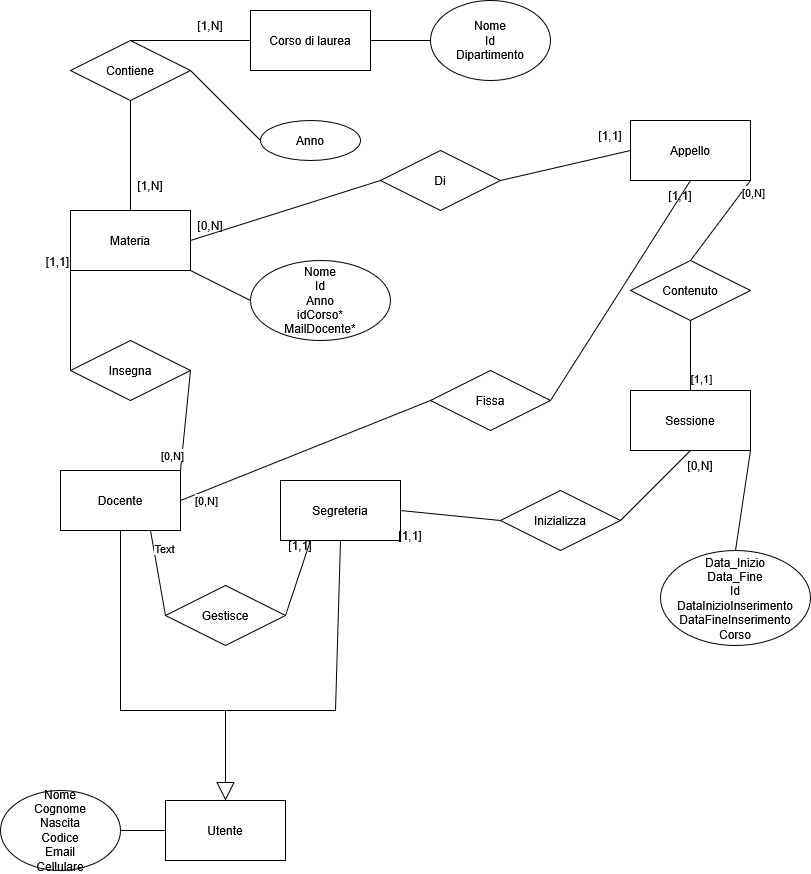
\includegraphics[width=0.92\linewidth]{uml-schema.png}
\caption{Schema dei dati del progetto (ER/UML). Si notino la gerarchia
\emph{IS-A} \textsc{Docente}/\textsc{Segreteria}~$\rightarrow$~\textsc{Utente} e
le relazioni \emph{Contiene}, \emph{Insegna}, \emph{Di}, \emph{Contenuto},
\emph{Fissa}, \emph{Inizializza}, \emph{Gestisce}.}
\label{fig:uml}
\end{figure}

WebML suggerisce di classificare gli oggetti in quattro tipi di sottoschema; il
progetto vi si mappa così:

\begin{description}[leftmargin=1.6em,style=nextline]
  \item[Core] gli oggetti informativi principali: \textsc{Corso di laurea},
        \textsc{Insegnamento}, \textsc{Sessione}, \textsc{Appello}. Sono le entità
        attorno a cui ruota lo schema.
  \item[Personalizzazione] descrive le proprietà degli utenti: i profili
        \textsc{Docente} e \textsc{Segreteria} sono \emph{sotto-classi IS-A} di
        \textsc{Utente}, esattamente il ``sottoschema di personalizzazione'' del
        corso. La linea guida WebML \textemdash{} \emph{inserire l'identificatore
        dell'utente nelle rotte che estraggono dati collegati all'utente}
        \textemdash{} è realizzata dalle rotte \code{/mine} e \code{/me}, dal
        metodo \code{findByUserId} dei repository e dal fatto che, creando un
        appello, il docente è forzato all'utente autenticato.
  \item[Interconnessione] le associazioni semantiche tra entità core
        (\emph{Insegnamento$\to$Corso}, \emph{Appello$\to$Sessione}, ecc.).
        Guidano i ``link'' di navigazione e, lato dati, la regola di buona
        progettazione applicata è il vincolo \code{onDelete: RESTRICT}: non si
        elimina un'entità finché ha entità collegate.
  \item[Accesso] gli oggetti ausiliari di categorizzazione/ricerca. Nel progetto
        sono minimali (es.\ i filtri per corso/docente sugli insegnamenti).
\end{description}

Una linea guida del corso particolarmente evidente è quella sulle \textbf{entità
deboli / componenti part-of}: la loro creazione avviene \emph{contestualmente}
all'entità core (``fusione delle rotte di creazione'') e la cancellazione della
core comporta una cancellazione a cascata. Nel progetto questo è il pattern di
creazione \textbf{atomica} di \textsc{Utente}~+~profilo (un solo endpoint
\code{POST /teachers} crea entrambi, con \emph{rollback} in caso di errore) e la
relazione \code{onDelete: CASCADE} tra profilo e utente.

\section{Progettazione dell'ipertesto}
\label{sec:webml-ipertesto}
La progettazione dell'ipertesto modella il front-end. Il concetto fondamentale è
la \textbf{site view}: una ``vista sul sito'' per ciascun gruppo utente. Nel
progetto la site view si concretizza nel \textbf{rendering condizionato al
ruolo}: navbar filtrata (voci \code{segreteriaOnly}), dashboard diversa per
Docente e Segreteria, scelta tra \code{/mine} e la lista completa. Le aree si
dividono in \textbf{pubbliche} (il login) e \textbf{private} (tutto il resto,
dietro \code{ProtectedRoute}).

\paragraph{Progetto coarse: aree e primitive.} Si individuano le \emph{aree}
(insiemi coesi di pagine) e le si descrive con le primitive del corso. Le aree
del progetto \textemdash{} Esami, Sessioni, Insegnamenti, Corsi di laurea,
Docenti, Segretari, Area personale \textemdash{} usano le primitive
\code{Core(\ldots)} per la pubblicazione dei contenuti e
\code{Create}/\code{Modify}/\code{Delete} per le operazioni; in particolare la
creazione di un appello (che collega materia e sessione) e quella di un docente
(\textsc{Utente}~+~profilo) sono istanze della primitiva
\code{Create\&Connect}.

\paragraph{Progetto dettagliato: pagine, visibilità, unità e link.} Le \emph{aree}
si suddividono in \textbf{pagine}, che diventano i componenti React
\file{*.page.tsx}. La \emph{visibilità} delle pagine del corso si ritrova
puntualmente:
\begin{itemize}[leftmargin=1.4em]
  \item \textbf{Home} (\emph{H}): la rotta \code{/} (dashboard col calendario),
        ``su cui si atterra dopo il login'';
  \item \textbf{Landmark} (\emph{L}): le pagine globalmente raggiungibili da ogni
        altra \textemdash{} sono le voci della \textbf{navbar}. Il professore dice
        esplicitamente che il raggruppamento di pagine landmark ``determina la
        navbar del sito'';
  \item \textbf{Interne}: le pagine raggiungibili solo via link espliciti, come i
        form \code{create}/\code{edit}.
\end{itemize}

Le \textbf{unità di contenuto} (Details, SimpleList, List, Form\ldots) si mappano
sui componenti di visualizzazione: una \emph{List} è la tabella di una pagina-lista,
un \emph{Form} è una pagina di creazione/modifica. I \textbf{link} si distinguono
in \emph{non contestuali} (la navbar, che non trasporta contesto) e
\emph{contestuali} (che trasportano un parametro): nel progetto il click su un
giorno verde del calendario apre il form già precompilato passando i dati in
query-string, e il pulsante ``Modifica'' porta all'\code{edit} con l'\code{:id}.
Le primitive di \textbf{login/logout} sono le pagine omonime; i \textbf{parametri
di contesto} (lo ``stato'' della pagina) sono gestiti con \code{useSearchParams} e
\code{useParams}.

\paragraph{La mappatura WebML$\,\rightarrow\,$React.} La tabella riassume la
corrispondenza adottata (ripresa anche nel capitolo conclusivo).

\begin{table}[h]
\centering
\renewcommand{\arraystretch}{1.25}
\begin{tabularx}{\linewidth}{@{}lX@{}}
\toprule
\textbf{Primitiva WebML} & \textbf{Realizzazione React} \\
\midrule
Site view (per gruppo utente) & rendering condizionato a \code{user.role} \\
Area / pagina landmark        & voce della navbar (\code{AppLayout}) \\
Pagina                        & componente \file{xxx.page.tsx} \\
Home page (H)                 & rotta \code{/} (dashboard) \\
Pagina interna                & form \code{create}/\code{edit} (link espliciti) \\
Unità di vista (List/Details) & tabella/elenco nel componente \\
Unità Form + Operation (CUD)  & pagine-form + funzioni di scrittura in \file{*.api.ts} \\
Create\&Connect               & creazione con FK (es.\ \textsc{Utente}+profilo) \\
Personalization               & rotte \code{/mine}, \code{/me}; filtro per utente \\
Link non contestuale          & navbar \\
Link contestuale / parametri  & \code{navigate} con query/\code{:id}; \code{useSearchParams}/\code{useParams} \\
Login/logout                  & pagine \file{login}/\file{logout} \\
Area pubblica / privata        & fuori / dentro \code{ProtectedRoute} \\
\bottomrule
\end{tabularx}
\caption{Corrispondenza tra primitive WebML e costrutti React del progetto.}
\label{tab:webml-react}
\end{table}

In sintesi, la struttura del codice non è arbitraria: deriva dal modello WebML.
I capitoli seguenti descrivono l'\emph{implementazione} di questo progetto.

% =====================================================================
\chapter{Backend: avvio, configurazione e modello dei dati}
\label{cap:backend}
% =====================================================================

Questo capitolo descrive come il backend NestJS si avvia, come è configurato il
database e come è strutturato il modello dei dati persistente. I capitoli
successivi entreranno nella logica applicativa (autenticazione e dominio).

\section{Il bootstrap dell'applicazione (\texttt{main.ts})}
Il file \file{apps/api/src/main.ts} è il punto d'ingresso del server: crea
l'istanza Nest a partire da \code{AppModule} e ne configura il comportamento
globale prima di mettersi in ascolto.

\begin{lstlisting}[caption={Estratto di \file{apps/api/src/main.ts}.}]
async function bootstrap() {
  const app = await NestFactory.create(AppModule);
  app.setGlobalPrefix('api');               // tutte le rotte sotto /api

  // Nessuna risposta API deve essere messa in cache dal browser
  app.use((_req, res, next) => {
    res.setHeader('Cache-Control', 'no-store');
    next();
  });

  app.enableCors({                          // il frontend gira su un'altra porta
    origin: process.env.CORS_ORIGIN ?? 'http://localhost:4200',
    credentials: true,
  });

  app.useGlobalPipes(new ValidationPipe({   // validazione+trasformazione DTO
    whitelist: true, forbidNonWhitelisted: true,
    transform: true, transformOptions: { enableImplicitConversion: true },
  }));

  app.useGlobalInterceptors(new ClassSerializerInterceptor(app.get(Reflector)));

  // Swagger su /api/docs
  const document = SwaggerModule.createDocument(app, config);
  SwaggerModule.setup('api/docs', app, document);

  await app.listen(process.env.PORT || 3000);
}
\end{lstlisting}

Le configurazioni globali, con la loro motivazione:

\begin{description}[leftmargin=1.6em,style=nextline]
  \item[Prefisso globale \code{/api}] tutte le rotte sono servite sotto
        \code{/api} (es. \code{/api/auth/login}). Tiene separato lo spazio delle
        API da eventuali risorse statiche.
  \item[\code{Cache-Control: no-store}] aggiunto a \emph{ogni} risposta. Senza di
        esso il solo \emph{ETag} di Express potrebbe far riusare al browser una
        copia vecchia di una lista (ad es. mostrare una sessione già eliminata
        sul server). È una correzione mirata a un problema osservato di cache.
  \item[CORS] abilita le richieste cross-origin dal frontend (porta 4200) verso
        l'API (porta 3333), poiché sono su origini diverse.
  \item[\code{ValidationPipe} globale] con \code{whitelist} (rimuove i campi non
        dichiarati nei DTO), \code{forbidNonWhitelisted} (rifiuta con 400 i campi
        sconosciuti), \code{transform} e \code{enableImplicitConversion}
        (converte automaticamente stringhe in numeri/date secondo il tipo del
        DTO). È il motore che fa girare i decoratori \code{class-validator} dei
        DTO. Le conseguenze: corpi di richiesta ``puliti'' e tipizzati, e
        validazione dichiarativa centralizzata.
  \item[\code{ClassSerializerInterceptor}] applica le regole di
        \code{class-transformer} in uscita; in particolare onora il decoratore
        \code{@Exclude()} sul campo \code{passwordHash} dell'utente, così l'hash
        non finisce mai nelle risposte serializzate.
  \item[Swagger] genera la documentazione interattiva delle API, raggiungibile su
        \code{http://localhost:<PORT>/api/docs}, con schema \emph{Bearer} per
        provare le rotte protette.
\end{description}

\section{Composizione del modulo radice (\texttt{AppModule})}
Coerentemente con la scelta di tenere l'app ``sottile'', \code{AppModule} si
limita a importare i moduli di dominio definiti nelle librerie:

\begin{lstlisting}[caption={\file{apps/api/src/app/app.module.ts}.}]
@Module({
  imports: [ServerUsersModule, DatabaseModule,
            ServerAuthModule, ServerExamPlanningModule],
  controllers: [AppController],
  providers: [AppService],
})
export class AppModule {}
\end{lstlisting}

Ogni modulo importato è una libreria autonoma: \code{DatabaseModule} apre la
connessione al database, \code{ServerUsersModule} e \code{ServerAuthModule}
gestiscono utenti e autenticazione, \code{ServerExamPlanningModule} raccoglie
tutte le entità di dominio. NestJS, tramite la \emph{dependency injection},
risolve le dipendenze tra questi moduli all'avvio.

\section{La configurazione del database (\texttt{DatabaseModule})}
La libreria \code{@org/database} configura TypeORM su PostgreSQL leggendo i
parametri dal file \file{.env}. Una piccola funzione \code{requireEnv} fa
fallire l'avvio con un messaggio chiaro se manca una variabile obbligatoria,
invece di proseguire con una connessione incompleta.

\begin{lstlisting}[caption={\file{libs/database/src/lib/database.module.ts}.}]
function requireEnv(name: string): string {
  const v = process.env[name];
  if (!v) throw new Error(`Variabile d'ambiente obbligatoria mancante: ${name}`);
  return v;
}

@Module({
  imports: [TypeOrmModule.forRoot({
    type: 'postgres',
    host: requireEnv('PG_HOST'),
    port: Number(requireEnv('PG_PORT')),
    username: requireEnv('PG_USERNAME'),
    password: requireEnv('PG_PASSWORD'),
    database: requireEnv('PG_DATABASE'),
    autoLoadEntities: true,   // registra le entità dai feature module
    synchronize: true,        // allinea lo schema al codice (solo sviluppo!)
  })],
  exports: [TypeOrmModule],
})
export class DatabaseModule {}
\end{lstlisting}

Due opzioni meritano attenzione:

\begin{itemize}[leftmargin=1.4em]
  \item \code{autoLoadEntities: true} \textemdash{} le entità non vanno elencate
        a mano qui: ogni feature module le registra con
        \code{TypeOrmModule.forFeature([\ldots])} e TypeORM le carica
        automaticamente.
  \item \code{synchronize: true} \textemdash{} all'avvio TypeORM allinea lo
        schema del database alle entità del codice. È comodissimo in sviluppo
        (niente migrazioni manuali) ma \textbf{non va usato in produzione},
        perché può alterare le tabelle in modo distruttivo.
\end{itemize}

\begin{table}[h]
\centering
\renewcommand{\arraystretch}{1.2}
\begin{tabularx}{\linewidth}{@{}lX@{}}
\toprule
\textbf{Variabile} & \textbf{Significato} \\
\midrule
\code{PORT}        & Porta di ascolto dell'API (il \file{.env} usa 3333; default 3000). \\
\code{PG\_HOST}    & Host PostgreSQL. \\
\code{PG\_PORT}    & Porta PostgreSQL. \\
\code{PG\_USERNAME}& Utente del database. \\
\code{PG\_PASSWORD}& Password del database. \\
\code{PG\_DATABASE}& Nome del database. \\
\code{SECRET\_KEY} & Segreto per la firma dei token JWT. \\
\bottomrule
\end{tabularx}
\caption{Variabili d'ambiente lette dal \file{.env}.}
\end{table}

\section{Il modello dei dati}
Il dominio è rappresentato da otto entità TypeORM. La figura~\ref{fig:er}
sintetizza le relazioni; le sezioni successive ne descrivono i dettagli.

\begin{figure}[h]
\centering
\begin{tikzpicture}[
  ent/.style={draw=accent!50,rounded corners=3pt,fill=accent!6,
    font=\footnotesize\bfseries,minimum height=0.85cm,minimum width=2.3cm,align=center},
  rel/.style={-{Latex[length=2mm]},thick,accent!70!black,font=\scriptsize},
  node distance=1.1cm and 1.7cm,
]
  \node[ent] (user) {User};
  \node[ent,below left=1.2cm and 0.6cm of user] (teacher) {Teacher};
  \node[ent,below right=1.2cm and 0.6cm of user] (sec) {Secretariat};
  \node[ent,below=2.6cm of teacher] (subject) {Subject};
  \node[ent,left=of subject] (course) {DegreeCourse};
  \node[ent,below=2.6cm of sec] (exam) {Exam};
  \node[ent,right=of exam] (session) {ExamSession};

  \draw[rel] (teacher) -- node[left]{1:1} (user);
  \draw[rel] (sec) -- node[right]{1:1} (user);
  \draw[rel] (subject) -- node[above]{N:1} (course);
  \draw[rel] (subject) -- node[right]{N:1} (teacher);
  \draw[rel] (exam) -- node[below]{N:1} (subject);
  \draw[rel] (exam) -- node[above]{N:1} (session);
  \draw[rel] (exam.north) to[bend right=12] node[right]{N:1} (teacher.south east);
\end{tikzpicture}
\caption{Relazioni tra le entità del dominio. \code{Teacher} e
\code{Secretariat} estendono un \code{User} (1:1, cascade); \code{Subject}
appartiene a un \code{DegreeCourse} e a un \code{Teacher}; \code{Exam} collega
\code{Subject}, \code{ExamSession} e \code{Teacher}.}
\label{fig:er}
\end{figure}

\subsection{Convenzioni comuni}
Tutte le entità di dominio condividono alcune convenzioni:

\begin{itemize}[leftmargin=1.4em]
  \item la \textbf{chiave primaria} è una colonna \code{id} auto-generata, ma
        nel codice è esposta con un nome parlante (\code{degreeCourseId},
        \code{subjectId}, \code{examId}\ldots) tramite
        \code{@PrimaryGeneratedColumn(\{ name: 'id' \})};
  \item le relazioni verso ``il padre'' sono \code{@ManyToOne} con
        \code{eager: true} (la relazione è sempre caricata insieme all'entità) e
        \code{onDelete: 'RESTRICT'} (non si può cancellare il padre se esistono
        figli);
  \item i vincoli di unicità ``di dominio'' sono espressi con \code{@Unique([...])}
        o \code{unique: true} sulla colonna.
\end{itemize}

\subsection{User, Teacher, Secretariat}
\code{UserEntity} (tabella \code{users}) è la base dell'autenticazione: ha
\code{name}, \code{email} (univoca, è l'identificativo di login),
\code{passwordHash} (hash bcrypt, annotato \code{@Exclude()} per non uscire mai
nelle risposte) e \code{role} (enum \code{UserRole}, default \code{DOCENTE}).

\code{TeacherEntity} e \code{SecretariatEntity} sono i \emph{profili}: ciascuno
ha una relazione \code{@OneToOne} verso \code{UserEntity} con
\code{onDelete: 'CASCADE'} (eliminando l'utente cade anche il profilo) ed
\code{eager: true}. La separazione utente/profilo permette di tenere le
credenziali in un'unica tabella e i dati specifici del ruolo altrove. Il docente
possiede inoltre gli insegnamenti (\code{@OneToMany} verso \code{Subject}) e gli
appelli (\code{@OneToMany} verso \code{Exam}); il segretario non possiede
risorse proprie perché amministra quelle altrui.

\subsection{DegreeCourse e Subject}
\code{DegreeCourseEntity} (\code{degree\_courses}) ha \code{name} (univoco),
\code{yearsDuration} (durata in anni, usata per validare l'anno degli
insegnamenti) e \code{department}.

\code{SubjectEntity} (\code{subjects}) ha \code{name}, \code{year}, \code{cfu}, e
due \code{@ManyToOne} obbligatori verso \code{DegreeCourse} e \code{Teacher}. Il
vincolo \code{@Unique(['name','degreeCourse'])} impedisce due insegnamenti con
lo stesso nome nello stesso corso.

\begin{lstlisting}[caption={Vincolo e relazioni di \file{subject.entity.ts} (estratto).}]
@Entity('subjects')
@Unique(['name', 'degreeCourse'])
export class SubjectEntity {
  @PrimaryGeneratedColumn({ name: 'id' }) subjectId: number;
  @Column() name: string;
  @Column() year: number;
  @Column() cfu: number;

  @ManyToOne(() => DegreeCourseEntity, (dc) => dc.subjects,
    { nullable: false, eager: true, onDelete: 'RESTRICT' })
  degreeCourse: DegreeCourseEntity;

  @ManyToOne(() => TeacherEntity, (t) => t.subjects,
    { nullable: false, eager: true, onDelete: 'RESTRICT' })
  teacher: TeacherEntity;
}
\end{lstlisting}

\subsection{ExamSession ed Exam}
\code{ExamSessionEntity} (\code{exam\_sessions}) ha \code{name} (univoco) e
\emph{quattro} date: \code{startDate}/\code{endDate} (periodo in cui si svolgono
gli appelli) e \code{planningStartDate}/\code{planningEndDate} (finestra entro
cui i docenti possono pianificare). Questa distinzione è il cuore della regola
``il docente pianifica solo a finestra aperta''.

\code{ExamEntity} (\code{exams}) ha \code{date}, \code{startHour},
\code{endHour}, \code{type} (enum \code{ExamType}: orale/scritto),
\code{roomType} (enum \code{RoomType}: aula standard o laboratori specializzati)
e tre \code{@ManyToOne} verso \code{Subject}, \code{ExamSession} e
\code{Teacher}. Il vincolo \code{@Unique(['date','subject'])} impedisce due
appelli della stessa materia nello stesso giorno (le altre regole, come il
conflitto ``corso+anno+giorno'', sono applicate dal service perché troppo
articolate per un solo vincolo SQL).

\section{Lo script di \emph{seed}}
Il file \file{apps/api/src/seed.ts} popola il database con dati di prova
coerenti: account (un segretario e due docenti), corsi, insegnamenti e
soprattutto tre sessioni \emph{passata}, \emph{corrente} e \emph{futura} con i
relativi appelli. Serve perché, attraverso l'API, un esame può essere creato
solo dal docente e solo dentro la finestra di pianificazione: dall'interfaccia
non si potrebbero quindi inserire appelli di sessioni passate. Lo script apre un
\emph{application context} di Nest e scrive direttamente tramite il
\code{DataSource} di TypeORM (CRUD puro), \textbf{bypassando} le regole di
dominio dei service.

È \textbf{idempotente} (logica \emph{find-or-create} per nome/email): può essere
rieseguito senza creare duplicati. Si lancia con \code{npm run seed} (richiede
PostgreSQL avviato e le variabili del \file{.env}). La password di tutti gli
account di prova è \code{Password1!}.

% =====================================================================
\chapter{Sicurezza e autenticazione}
\label{cap:auth}
% =====================================================================

L'autenticazione è basata su \textbf{token JWT} emessi al login e verificati a
ogni richiesta successiva, con \textbf{Passport} come libreria di strategie e un
sistema di \textbf{guard} e \textbf{decoratori} per l'autorizzazione per ruolo.
La materia è ripartita su tre librerie: \code{@server/security} (i mattoni
riusabili di autorizzazione), \code{@server/auth} (login, emissione token,
strategie) e \code{@server/users} (gli account e il loro CRUD).

\section{La libreria \texttt{@server/security}}
Raccoglie i componenti di autorizzazione condivisi da tutti i moduli.

\paragraph{L'enum \code{UserRole}.} I due ruoli del sistema. Vive qui (e non in
\code{@server/users}) per rompere una dipendenza circolare tra i moduli utenti e
sicurezza.

\paragraph{\code{JwtAuthGuard}.} Estende l'\code{AuthGuard('jwt')} di Passport:
protegge una rotta richiedendo un token valido. Estrae il token dall'header
\code{Authorization}, lo verifica e popola \code{request.user}; senza token
valido risponde \textbf{401}.

\paragraph{\code{RolesGuard}.} Autorizza per ruolo e va usato \emph{dopo} il
\code{JwtAuthGuard}. Legge, tramite il \code{Reflector}, i ruoli dichiarati con
\code{@Roles(\ldots)} sulla rotta e consente l'accesso solo se l'utente corrente
ne possiede uno; altrimenti \textbf{403}.

\begin{lstlisting}[caption={\file{roles.guard.ts} (estratto).}]
canActivate(context: ExecutionContext): boolean {
  const requiredRoles = this.reflector.getAllAndOverride<UserRole[]>(
    ROLES_KEY, [context.getHandler(), context.getClass()]);
  if (!requiredRoles || requiredRoles.length === 0) return true; // rotta libera
  const user = context.switchToHttp().getRequest().user;
  if (!user) throw new ForbiddenException('Utente non presente nella richiesta');
  if (!requiredRoles.includes(user.role))
    throw new ForbiddenException('Permessi insufficienti');
  return true;
}
\end{lstlisting}

\paragraph{I decoratori \code{@Roles(\ldots)} e \code{@CurrentUser()}.}
\code{@Roles} salva i ruoli ammessi nei metadati della rotta (sotto la chiave
\code{ROLES\_KEY}) che il \code{RolesGuard} poi rilegge. \code{@CurrentUser()} è
un \emph{param decorator} che estrae \code{request.user} e lo passa come
argomento al metodo del controller, evitando di leggere a mano la request:

\begin{lstlisting}[caption={Uso combinato di guard e decoratori su una rotta.}]
@Post()
@UseGuards(JwtAuthGuard, RolesGuard)
@Roles(UserRole.DOCENTE)
@ApiBearerAuth()
create(@Body() dto: CreateExamDto, @CurrentUser() user: AuthenticatedUser) {
  return this.service.createOne(dto, user);
}
\end{lstlisting}

\section{La libreria \texttt{@server/auth}}
Configura Passport e l'emissione/verifica dei token, ed espone le rotte di
login e registrazione.

\paragraph{Il modulo.} \code{ServerAuthModule} importa \code{ServerUsersModule}
(per leggere/creare utenti), \code{PassportModule} e \code{JwtModule}; quest'ultimo
è configurato con il segreto \code{SECRET\_KEY} e una scadenza dei token di
\textbf{24 ore}. Registra come provider le due strategie e il service.

\paragraph{Le due strategie Passport.}
\begin{description}[leftmargin=1.6em,style=nextline]
  \item[\code{LocalStrategy}] usata al login dal \code{LocalAuthGuard}. È
        configurata con \code{usernameField: 'email'} (l'identificativo è
        l'email, non lo \emph{username} di default) e delega la verifica delle
        credenziali al service.
  \item[\code{JwtStrategy}] usata dal \code{JwtAuthGuard}. Estrae il token come
        \emph{Bearer} dall'header, ne verifica la firma con \code{SECRET\_KEY} e
        rifiuta i token scaduti; dal payload ricostruisce l'oggetto
        \code{AuthenticatedUser} che finisce in \code{request.user}.
\end{description}

\paragraph{Il service.} \code{ServerAuthService} contiene la logica vera:

\begin{lstlisting}[caption={\file{auth.service.ts} (estratto).}]
async validateUser(email: string, password: string): Promise<AuthenticatedUser> {
  const user = await this.usersService.findByEmail(email);
  if (!user) throw new UnauthorizedException('Credenziali non valide');
  const ok = await bcrypt.compare(password, user.passwordHash);
  if (!ok) throw new UnauthorizedException('Credenziali non valide');
  const { passwordHash, ...result } = user;   // mai esporre l'hash
  return result;
}

async login(user: AuthenticatedUser): Promise<AuthResponse> {
  const payload = { sub: user.id, name: user.name, email: user.email, role: user.role };
  return { access_token: await this.jwtService.signAsync(payload), user };
}
\end{lstlisting}

Due aspetti di sicurezza degni di nota:
\begin{itemize}[leftmargin=1.4em]
  \item \textbf{nessuna \emph{user enumeration}}: sia per email inesistente sia
        per password errata viene lanciato lo stesso \textbf{401} con lo stesso
        messaggio ``Credenziali non valide'', così un attaccante non può dedurre
        quali email siano registrate;
  \item l'\textbf{hash della password non esce mai}: viene rimosso con
        destrutturazione (\code{const \{ passwordHash, ...result \} = user}) e in
        più è marcato \code{@Exclude()} sull'entità.
\end{itemize}

Il \textbf{payload} del JWT è \code{\{ sub, name, email, role \}} (la convenzione
JWT vuole \code{sub} = \emph{subject} = id utente). Le interfacce
\code{JwtPayload}, \code{AuthenticatedUser} e \code{AuthResponse} tipizzano
rispettivamente il contenuto del token, l'utente a runtime in \code{request.user}
e la risposta di login/registrazione (\code{\{ access\_token, user \}}).

\paragraph{Le rotte di autenticazione.}
\begin{description}[leftmargin=1.6em,style=nextline]
  \item[\code{POST /auth/login}] rotta \textbf{pubblica}: il \code{LocalAuthGuard}
        valida email+password e popola \code{req.user}; il controller restituisce
        token e utente.
  \item[\code{POST /auth/register}] riservata alla \textbf{Segreteria}
        (\code{JwtAuthGuard + RolesGuard + @Roles(SEGRETERIA)}). Crea un utente
        ``nudo'' (senza profilo) e ne restituisce subito il token. Non è la via
        normale di onboarding (vedi sotto).
\end{description}

\section{La libreria \texttt{@server/users}}
Gestisce gli account. \code{ServerUsersService} si occupa dell'hashing
(\code{bcrypt}, 10 \emph{salt rounds}), del controllo di unicità dell'email
(\textbf{409} se già in uso) e della traduzione di ``non trovato'' in
\textbf{404}; delega l'accesso ai dati a \code{UsersRepository}, un wrapper di
puro CRUD sul \code{Repository<UserEntity>} di TypeORM. Il \code{ServerUsersController}
espone il CRUD utenti, quasi tutto riservato alla Segreteria, più la rotta
\code{GET /users/me} che restituisce il payload dell'utente autenticato
(\code{\{ id, name, email, role \}}).

\paragraph{Regole sulla password.} Definite dichiarativamente nel
\code{CreateUserDto} con \code{class-validator}: minimo 8 caratteri, almeno una
lettera maiuscola e almeno un simbolo tra \code{? \^{} ! \# @}. I messaggi di
errore sono in italiano.

\section{Il flusso di autenticazione e la policy di onboarding}
Mettendo insieme i pezzi, una richiesta autenticata segue questo percorso:

\begin{enumerate}[leftmargin=1.6em]
  \item il client invia \code{POST /api/auth/login} con email e password;
  \item \code{LocalAuthGuard}$\rightarrow$\code{LocalStrategy}$\rightarrow$
        \code{validateUser} verificano le credenziali; in caso positivo
        \code{login} firma un JWT e restituisce \code{\{ access\_token, user \}};
  \item il client conserva il token e lo invia nell'header
        \code{Authorization: Bearer <token>} a ogni chiamata successiva;
  \item sulle rotte protette il \code{JwtAuthGuard}$\rightarrow$\code{JwtStrategy}
        verificano il token e popolano \code{request.user}; dove serve, il
        \code{RolesGuard} controlla anche il ruolo.
\end{enumerate}

\paragraph{Onboarding reale.} È importante notare che \code{POST /auth/register}
e \code{POST /users} creano un utente \emph{senza profilo} e perciò \textbf{non}
sono la via normale per registrare gli account. La creazione reale avviene via
\code{POST /teachers} e \code{POST /secretariats} (riservate alla Segreteria):
ciascuna crea in modo \emph{atomico} l'utente \emph{e} il suo profilo, forzando
il ruolo lato server e facendo \emph{rollback} dell'utente se la creazione del
profilo fallisce. Questo meccanismo è descritto nel capitolo~\ref{cap:dominio}.

% =====================================================================
\chapter{Il pattern a livelli e la logica di dominio}
\label{cap:dominio}
% =====================================================================

Il cuore applicativo del backend è la libreria \code{@server/exam-planning}, che
contiene tutte le entità di dominio e la loro logica. Ogni entità segue la stessa
struttura a livelli; questo capitolo prima descrive il \emph{pattern} in
generale, poi entra nelle regole specifiche di ciascuna entità.

\section{Il pattern a quattro livelli}
Ogni feature di dominio è organizzata negli stessi quattro livelli, con
responsabilità nette. Questa uniformità rende il codice prevedibile: imparato un
modulo, si conoscono tutti.

\begin{figure}[h]
\centering
\begin{tikzpicture}[
  layer/.style={draw=accent!50,rounded corners=3pt,fill=accent!6,
    minimum width=11cm,minimum height=1.05cm,align=left,font=\small,inner sep=8pt},
  arr/.style={-{Latex[length=2.5mm]},thick,accent!70!black},
  node distance=0.55cm,
]
  \node[layer] (c) {\textbf{Controller}\quad routing, guard, \code{ParseIntPipe}, \code{@Body() dto}, Swagger};
  \node[layer,below=of c] (s) {\textbf{Service}\quad regole di dominio, 404, mapping errori DB, \code{toListItem}};
  \node[layer,below=of s] (r) {\textbf{Repository}\quad CRUD puro su \code{Repository<Entity>}, niente eccezioni HTTP};
  \node[layer,below=of r] (e) {\textbf{Entity / DTO / interface}\quad tabella, validazione input, forma di output};
  \draw[arr] (c) -- (s); \draw[arr] (s) -- (r); \draw[arr] (r) -- (e);
  \draw[arr,dashed,accent!50] (e.east) to[bend left=22] node[right,font=\scriptsize]{} (c.east);
\end{tikzpicture}
\caption{I quattro livelli di ogni feature di dominio e il flusso di una
richiesta dall'alto verso il basso.}
\end{figure}

\begin{description}[leftmargin=1.6em,style=nextline]
  \item[Repository (\file{xxx.repository.ts})] classe \code{@Injectable} che
        incapsula il \code{Repository<XxxEntity>} di TypeORM. Solo CRUD puro
        (\code{findAll}, \code{findById}, \code{createOne}, \code{updateOne},
        \code{deleteOne}) più eventuali query di supporto. Usa \code{find}/
        \code{findOne} (non il \emph{QueryBuilder}) così che le relazioni
        \code{eager} siano sempre caricate. Non lancia eccezioni HTTP: ritorna
        \code{null}/\code{boolean} per segnalare assenza o esito.
  \item[Service (\file{xxx.service.ts})] inietta il repository \emph{custom} (non
        \code{@InjectRepository}). Traduce \code{null}$\rightarrow$
        \code{NotFoundException}, racchiude le scritture in \code{try/catch} +
        \code{handleDatabaseError}, e possiede le regole di dominio. Espone
        sempre una forma ``piatta'' \code{XxxListItem}, mai l'entità TypeORM: un
        \code{toListItem(entity)} privato fa la conversione. Quando una lettura
        serve internamente come entità, il service usa un privato
        \code{getEntityById} (\emph{non} il pubblico \code{findById}, che ora
        ritorna un list-item).
  \item[List-item (\file{interfaces/xxx-list-item.interface.ts})] l'interfaccia
        della forma esposta al client (e condivisa col frontend, vedi
        \S\ref{sec:barrel}). Una per entità, usata sia per la lista sia per il
        dettaglio.
  \item[Controller (\file{xxx.controller.ts})] routing + guard
        (\code{JwtAuthGuard}, \code{RolesGuard} + \code{@Roles}) +
        \code{ParseIntPipe} sui parametri \code{:id}, Swagger minimale
        (\code{@ApiTags}, \code{@ApiBearerAuth}). Usa \code{@Body() dto: XxxDto}
        (validato dal \code{ValidationPipe} globale) e \emph{non} annota il tipo
        di ritorno: eredita il list-item dal service.
\end{description}

\paragraph{Perché un list-item e non l'entità.} Esporre direttamente l'entità
TypeORM avrebbe due difetti: trascinerebbe nel JSON le relazioni \code{eager}
(con campi sensibili come \code{user.passwordHash}) e legherebbe il contratto
dell'API alla struttura del database. Il \code{toListItem} produce invece una
forma stabile e ``piatta'': rinomina \code{xxxId}$\rightarrow$\code{id}, annida
le chiavi esterne come \code{\{ id, name \}} e rimuove i campi sensibili. Esempio:

\begin{lstlisting}[caption={\code{toListItem} degli esami (estratto).}]
private toListItem(exam: ExamEntity): ExamListItem {
  return {
    id: exam.examId,
    date: this.toIso(exam.date),       // 'YYYY-MM-DD'
    startHour: exam.startHour, endHour: exam.endHour,
    roomType: exam.roomType, type: exam.type,
    subject: { id: exam.subject.subjectId, name: exam.subject.name },
    examSession: { id: exam.examSession.examSessionId, name: exam.examSession.name },
    teacher: { id: exam.teacher.teacherId, name: exam.teacher.user.name },
  };
}
\end{lstlisting}

\section{Il barrel \texttt{index.ts} e la condivisione col frontend}
\label{sec:barrel}
Il file \file{libs/server/exam-planning/src/index.ts} è la \emph{superficie
pubblica} della libreria: ri-esporta il modulo NestJS \emph{più} tutte le
entità, i DTO, gli enum (\code{ExamType}, \code{RoomType}) e le interfacce
list-item. Grazie a questo, il frontend può scrivere

\begin{lstlisting}[caption={Import dei tipi del backend nel frontend.}]
import type { ExamListItem, CreateExamDto } from '@server/exam-planning';
\end{lstlisting}

riusando \emph{gli stessi tipi} del backend. Si usa \code{import type} per
importare solo i \emph{tipi} (cancellati a compile-time) ed evitare di trascinare
nel bundle del browser il codice runtime di \code{class-validator}/Swagger. È un
beneficio diretto del monorepo: un unico contratto, tipizzato, condiviso tra i
due lati.

\section{I DTO: validazione e trasformazione dell'input}
Il corpo di ogni richiesta di scrittura è descritto da un \textbf{DTO} (\emph{Data
Transfer Object}): una classe i cui campi portano i decoratori di
\code{class-validator} (es. \code{@IsString}, \code{@IsInt}, \code{@IsEmail},
\code{@IsOptional}) e gli \code{@ApiProperty} per Swagger. Il
\code{ValidationPipe} globale li fa rispettare automaticamente, scartando i
campi non dichiarati e convertendo i tipi. I messaggi d'errore sono in italiano.

Per evitare duplicazioni, gli \code{UpdateXxxDto} \textbf{non} riscrivono i campi
ma derivano dal corrispondente \code{CreateXxxDto} con i \emph{mapped types} di
\code{@nestjs/swagger}: \code{PartialType} rende tutti i campi opzionali (così il
\code{PATCH} può essere parziale), e \code{OmitType} ne esclude alcuni. Si usano
le versioni di \code{@nestjs/swagger} (non di \code{@nestjs/mapped-types}) perché
preservano anche i metadati Swagger.

\begin{lstlisting}[caption={DTO Create/Update (estratti).}]
export class CreateDegreeCourseDto {
  @ApiProperty({ example: 'Ingegneria Informatica', maxLength: 255 })
  @IsString({ message: 'Il nome del corso di laurea deve essere una stringa di testo' })
  @IsNotEmpty({ message: 'Il nome del corso di laurea è obbligatorio' })
  @MaxLength(255) name: string;

  @ApiProperty({ default: 3, required: false })
  @IsOptional() @IsInt() @Min(1) @Max(6)   // opzionale, default 3 sul DB
  yearsDuration?: number;

  @IsString() @IsNotEmpty() department: string;
}

// Tutti i campi opzionali
export class UpdateDegreeCourseDto extends PartialType(CreateDegreeCourseDto) {}

// Tutti opzionali E senza 'password' (si cambia per altra via)
export class UpdateUserDto extends PartialType(
  OmitType(CreateUserDto, ['password'] as const)) {}
\end{lstlisting}

Un principio di sicurezza importante: i \textbf{campi sensibili non compaiono mai}
nei DTO rivolti al client. Il \code{role}, ad esempio, non è nel
\code{CreateTeacherDto}/\code{CreateSecretariatDto}: è \emph{forzato lato server}
nel service (cfr.\ la creazione atomica più avanti), così il client non può
auto-assegnarsi un ruolo.

\section{La gestione centralizzata degli errori del database}
Le scritture possono fallire per violazioni di vincoli del database. L'helper
\code{handleDatabaseError(error, fallback)} (in \file{database-error.helper.ts},
tipo di ritorno \code{never}) traduce i codici d'errore di PostgreSQL nelle
eccezioni HTTP appropriate:

\begin{table}[h]
\centering
\renewcommand{\arraystretch}{1.2}
\begin{tabular}{@{}lll@{}}
\toprule
\textbf{Codice PG} & \textbf{Significato} & \textbf{HTTP} \\
\midrule
23505 & unique\_violation        & 409 Conflict \\
23502 & not\_null\_violation     & 422 Unprocessable Entity \\
23503 & foreign\_key\_violation  & 400 Bad Request \\
23514 & check\_violation         & 422 Unprocessable Entity \\
23P01 & exclusion\_violation     & 409 Conflict \\
40001 / 40P01 & serialization / deadlock & 503 Service Unavailable \\
(altro) & ---                    & 500 Internal Server Error \\
\bottomrule
\end{tabular}
\caption{Mappatura codici PostgreSQL $\rightarrow$ eccezioni HTTP.}
\end{table}

Il pattern adottato nei service è: \code{try \{ \ldots \} catch (e) \{ if (e
instanceof NotFoundException) throw e; handleDatabaseError(e, '\ldots'); \}}.
Le eccezioni applicative (\code{NotFoundException}, \code{ForbiddenException}\ldots)
vengono rilanciate \emph{prima} di delegare all'helper, così non vengono
trasformate per errore in un 500. Avere \code{never} come tipo di ritorno
permette di usarlo come ultima istruzione del \code{catch} soddisfacendo il
controllo di tipo.

\paragraph{Unicità ``umana'' dei nomi.} Un vincolo \code{UNIQUE} di PostgreSQL
confronta i byte esatti: distingue maiuscole e spazi. L'helper
\file{name-normalize.helper.ts} fornisce \code{normalizeName} (trim + spazi
interni collassati, usato in salvataggio) e \code{nameKey} (chiave
case-insensitive per il confronto), così ``Programmazione Web'' e
``programmazione~~web~'' sono trattati come duplicati.

\section{Le rotte REST del dominio}
La tabella riassume gli endpoint principali e il ruolo richiesto. Il prefisso
globale \code{/api} è sottinteso.

\begin{table}[h]
\centering
\small
\renewcommand{\arraystretch}{1.15}
\begin{tabularx}{\linewidth}{@{}llX@{}}
\toprule
\textbf{Metodo \& rotta} & \textbf{Ruolo} & \textbf{Azione} \\
\midrule
\code{GET /degree-courses}        & SEGR & elenco corsi \\
\code{GET /degree-courses/mine}   & DOC  & i corsi del docente \\
\code{POST/PATCH/DELETE /degree-courses} & SEGR & CRUD corsi \\
\code{GET /subjects}              & SEGR/DOC & elenco insegnamenti (con filtri) \\
\code{GET /subjects/mine}         & DOC  & gli insegnamenti del docente \\
\code{POST/PATCH/DELETE /subjects}& SEGR & CRUD insegnamenti \\
\code{GET /exam-sessions}         & SEGR/DOC & elenco sessioni (lettura per entrambi) \\
\code{POST/PATCH/DELETE /exam-sessions} & SEGR & CRUD sessioni \\
\code{GET /exams}                 & SEGR & tutti gli appelli \\
\code{GET /exams/mine}            & DOC  & gli appelli del docente \\
\code{GET /exams/by-course-year}  & DOC  & appelli per corso+anno (calendario) \\
\code{POST /exams}                & DOC  & crea un appello \\
\code{PATCH/DELETE /exams/:id}    & SEGR/DOC & modifica/elimina (regole di proprietà) \\
\code{GET /teachers}, \code{POST /teachers} & SEGR & elenco / crea docente \\
\code{GET /teachers/me}           & DOC  & il proprio profilo \\
\code{PATCH/DELETE /teachers/:id} & SEGR/DOC & modifica/elimina (self per il docente) \\
\code{GET/POST /secretariats}     & SEGR & elenco / crea segretario \\
\code{PATCH/DELETE /secretariats/:id} & SEGR & solo il proprio profilo (self-only) \\
\bottomrule
\end{tabularx}
\caption{Endpoint REST del dominio e ruolo richiesto.}
\end{table}

\section{Logica per entità}

\subsection{Corsi di laurea}
Gestiti dalla Segreteria. Il service valida l'unicità ``umana'' del nome (via
\code{nameKey}) oltre al vincolo del DB, e \textbf{impedisce l'eliminazione} di un
corso che abbia insegnamenti collegati: poiché la FK è \code{RESTRICT}, controlla
\emph{proattivamente} il conteggio dei figli e risponde con un \textbf{409} dal
messaggio chiaro, invece del 400 generico da violazione di foreign key.

\subsection{Insegnamenti}
Il service coordina più repository. In creazione/aggiornamento:
risolve le FK (corso, docente) con 404 se assenti; valida che l'\code{year} sia
compreso tra 1 e \code{yearsDuration} del corso; verifica l'unicità del nome
\emph{all'interno} dello stesso corso. L'aggiornamento rivaluta queste regole sui
valori \emph{risultanti} (mix tra DTO e valori esistenti). Anche qui
l'eliminazione è bloccata (409) se esistono appelli collegati. La lettura
supporta filtri per corso e/o docente, e una rotta \code{/mine} per il docente.

\subsection{Sessioni d'esame}
Gestite dalla Segreteria. La validazione delle date impone:
\code{startDate < endDate}, \code{planningStartDate < planningEndDate} e
\code{planningEndDate $\le$ startDate} (la pianificazione si chiude prima che la
sessione inizi). Inoltre i \emph{periodi} \code{[startDate, endDate]} di due
sessioni \textbf{non possono sovrapporsi} (le finestre di pianificazione invece
sì). Le date ISO sono confrontate direttamente come stringhe. L'eliminazione è
bloccata (409) se la sessione ha appelli.

\subsection{Appelli (la logica più ricca)}
\label{sec:exam-rules}
Il service degli esami coordina quattro repository (esami, materie, sessioni,
docenti) e concentra le regole più articolate.

\paragraph{Creazione (solo Docente).} Risolve materia, sessione e il profilo
docente dell'utente corrente; verifica che la materia sia \emph{del} docente
(altrimenti 403); applica \code{validateExam} e salva, forzando il docente
all'utente autenticato.

\paragraph{La validazione \code{validateExam}.} È applicata sia in creazione sia
in modifica, e lancia alla prima regola violata:

\begin{enumerate}[leftmargin=1.6em]
  \item \code{startHour < endHour} (altrimenti 400);
  \item la data dev'essere compresa tra \code{startDate} e \code{endDate} della
        sessione (400);
  \item se l'utente è un Docente, ``oggi'' deve cadere nella finestra di
        pianificazione \code{[planningStartDate, planningEndDate]} (altrimenti
        403);
  \item la data non può essere sabato o domenica (400). Si usa \code{getUTCDay}
        sulla data ISO per non sfasare il giorno della settimana col fuso del
        server;
  \item nessun \textbf{conflitto corso+anno+giorno}: non può esistere un altro
        appello nello stesso giorno per lo stesso anno dello stesso corso di
        laurea (409). In modifica, l'esame corrente è escluso dal confronto;
  \item la stessa materia non può avere due appelli nella stessa sessione (409).
\end{enumerate}

\paragraph{Modifica ed eliminazione.} La Segreteria può modificare/eliminare
qualsiasi appello; il Docente solo i propri (403 altrimenti) e \textbf{non} se
l'appello è già passato (un esame è ``passato'' se la sua data è precedente a
oggi). La modifica rivaluta \code{validateExam} sui valori risultanti.

\paragraph{La rotta \code{by-course-year}.} Restituisce tutti gli appelli di un
dato corso+anno, di \emph{qualsiasi} docente. Serve al calendario del docente sia
per colorare di rosso i giorni ``occupati'' dalla regola di conflitto, sia per
mostrare \emph{quali} esami occupano un giorno in cui non può inserirne uno
proprio (anche se non ne è il titolare).

\subsection{Docenti e segretari (creazione atomica e \emph{self-only})}
La creazione di un docente o segretario coinvolge due tabelle (utente e profilo)
e dev'essere atomica:

\begin{lstlisting}[caption={Creazione atomica di un docente con rollback.}]
async createOne(dto: CreateTeacherDto): Promise<TeacherListItem> {
  dto.name = normalizeName(dto.name);
  const user = await this.usersService.create({ ...dto, role: UserRole.DOCENTE });
  try {
    return this.toListItem(await this.repository.createOne(user));
  } catch (error) {
    await this.usersService.removeUser(user.id).catch(() => undefined); // rollback
    handleDatabaseError(error, 'Errore durante la creazione del docente');
  }
}
\end{lstlisting}

Il ruolo è \textbf{forzato lato server} (\code{role: UserRole.DOCENTE} /
\code{SEGRETERIA}), non arriva mai dal client. Se la creazione del profilo
fallisce, l'utente appena creato viene rimosso, evitando account ``orfani''.

Sulle modifiche e cancellazioni valgono i controlli di proprietà:
\begin{itemize}[leftmargin=1.4em]
  \item un \textbf{Docente} può vedere/modificare/eliminare solo il proprio
        profilo e non può cambiarsi l'email; non è eliminabile se ha insegnamenti
        o appelli collegati (409). La Segreteria può gestire qualsiasi docente;
  \item un \textbf{Segretario} è \emph{self-only} su tutta la linea: può
        vedere/modificare/eliminare solo il proprio profilo, e nemmeno cambiarsi
        l'email. La Segreteria può crearne e elencarli.
\end{itemize}

% =====================================================================
\chapter{Il frontend React}
\label{cap:frontend}
% =====================================================================

Il frontend (\code{apps/ui}) è una \textbf{SPA} React costruita con Vite, con
routing client tramite React Router e stile Tailwind CSS. Segue la mappatura
WebML$\rightarrow$React del corso: le \emph{pagine} diventano componenti
\file{*.page.tsx}, le \emph{operazioni} verso il backend stanno in
\file{*.api.ts}, le \emph{aree landmark} sono le voci della navbar.

\section{Organizzazione del codice}
Il codice è organizzato \textbf{per feature}: ogni entità di dominio ha una
cartella sotto \file{src/features/} con le sue pagine e il suo client API. La
struttura tipica di una feature è:

\begin{itemize}[leftmargin=1.4em]
  \item \file{xxx.api.ts} \textemdash{} funzioni che chiamano il backend
        (fetch + gestione errori);
  \item \file{xxx.page.tsx} \textemdash{} la pagina-lista;
  \item \file{create-xxx.page.tsx}, \file{edit-xxx.page.tsx} \textemdash{} i form
        di creazione e modifica.
\end{itemize}

Accanto alle feature di dominio ci sono cartelle trasversali: \file{auth/}
(login, logout, rotta protetta, client di autenticazione), \file{shared/}
(infrastruttura HTTP comune), \file{layouts/} (il guscio con la navbar),
\file{calendar/} (il componente calendario) e \file{dashboard/} (la home).

\section{Avvio e routing}
Il file \file{main.tsx} monta l'app dentro un \code{<BrowserRouter>}. Il
componente \code{App} (\file{app/app.tsx}) dichiara tutte le rotte:

\begin{lstlisting}[caption={Struttura delle rotte (estratto di \file{app.tsx}).}]
<Routes>
  <Route path="/login"  element={<LoginPage />} />   {/* pubblica */}
  <Route path="/logout" element={<LogoutPage />} />

  {/* Gruppo protetto: ProtectedRoute (richiede token) + AppLayout (navbar) */}
  <Route element={<ProtectedRoute><AppLayout /></ProtectedRoute>}>
    <Route index element={<DashboardPage />} />       {/* home '/' */}
    <Route path="/exams" element={<ExamsPage />} />
    <Route path="/exams/new" element={<CreateExamPage />} />
    <Route path="/exams/:id/edit" element={<EditExamPage />} />
    {/* ...le altre entità... */}
    <Route path="/me" element={<ProfilePage />} />
  </Route>

  <Route path="*" element={<Navigate to="/" replace />} /> {/* fallback */}
</Routes>
\end{lstlisting}

Si nota la struttura a \textbf{due livelli}: le rotte pubbliche
(\code{/login}, \code{/logout}) e un \textbf{gruppo protetto} annidato sotto
\code{ProtectedRoute} + \code{AppLayout}. Tutte le pagine autenticate sono figlie
di questo gruppo e vengono iniettate nell'\code{<Outlet/>} del layout; qualsiasi
rotta sconosciuta rimanda alla home.

\paragraph{La rotta protetta.} \code{ProtectedRoute} è semplicissima: se in
\code{localStorage} non c'è il token, reindirizza a \code{/login}; altrimenti
mostra i figli.

\begin{lstlisting}[caption={\file{protected-route.tsx}.}]
export function ProtectedRoute({ children }: { children: ReactNode }) {
  const token = localStorage.getItem('access_token');
  if (!token) return <Navigate to="/login" replace />;
  return children;
}
\end{lstlisting}

\section{L'infrastruttura HTTP condivisa}
Tutte le chiamate passano da \file{features/shared/utils.api.ts}, che centralizza
tre cose: l'URL base del backend, gli header autenticati e la gestione degli
errori. Così ogni \file{*.api.ts} le riusa senza duplicarle.

\begin{lstlisting}[caption={\file{shared/utils.api.ts} (estratto).}]
export const API_URL = 'http://localhost:3333/api';

export function getAuthHeaders(): HeadersInit {
  const token = localStorage.getItem('access_token');
  return { 'Content-Type': 'application/json',
           ...(token ? { Authorization: `Bearer ${token}` } : {}) };
}

export async function handleApiError(response: Response): Promise<never> {
  let message = `Errore ${response.status}`;
  try {
    const body = await response.json();
    if (Array.isArray(body?.message)) message = body.message.join('\n');
    else if (typeof body?.message === 'string') message = body.message;
  } catch { /* corpo non-JSON: si tiene il default */ }
  throw new Error(message);
}
\end{lstlisting}

\code{handleApiError} merita attenzione: il backend NestJS restituisce un corpo
\code{\{ message: string | string[] \}}. Quando \code{message} è un \emph{array}
(tipico degli errori di \code{class-validator}, un messaggio per regola), li
unisce su più righe; quando è una stringa, la usa così com'è. In entrambi i casi
il messaggio mostrato all'utente è quello \emph{italiano} prodotto dal backend.

\section{L'autenticazione lato client}
\file{features/auth/auth.api.ts} implementa il login e le utilità sull'utente
corrente. Al login salva token e utente in \code{localStorage}; espone
\code{getCurrentUser()} (lettura sincrona, senza rete) usato dalle pagine per
conoscere il ruolo, e \code{logout()} che ripulisce lo storage.

\begin{lstlisting}[caption={\code{login} (estratto di \file{auth.api.ts}).}]
export async function login(email: string, password: string): Promise<CurrentUser> {
  const response = await fetch(`${API_URL}/auth/login`, {
    method: 'POST', headers: { 'Content-Type': 'application/json' },
    body: JSON.stringify({ email, password }),
  });
  if (!response.ok) await handleApiError(response);
  const data = await response.json();
  localStorage.setItem('access_token', data.access_token);
  localStorage.setItem('current_user', JSON.stringify(data.user));
  return data.user;
}
\end{lstlisting}

La \code{LoginPage} è un \emph{form controllato} (i valori dei campi vivono nello
\emph{state} React): al submit chiama \code{login} e, in caso di successo,
naviga alla home; in caso di errore mostra il messaggio del backend.

\section{Il layout e la navbar}
\code{AppLayout} è il guscio delle pagine autenticate: una navbar fissa in alto e
l'\code{<Outlet/>} per la pagina corrente. Le voci di menu sono dichiarate in un
array; alcune sono marcate \code{segreteriaOnly} e compaiono solo per la
Segreteria, applicando lato UI la stessa divisione di permessi del backend:

\begin{lstlisting}[caption={Voci di navbar e filtro per ruolo (estratto).}]
const navItems = [
  { to: '/exams', label: 'Esami' },
  { to: '/exam-sessions', label: 'Sessioni' },
  { to: '/subjects', label: 'Insegnamenti' },
  { to: '/degree-courses', label: 'Corsi di laurea' },
  { to: '/teachers', label: 'Docenti', segreteriaOnly: true },
  { to: '/secretariats', label: 'Segretari', segreteriaOnly: true },
];
const isSegreteria = user?.role === 'SEGRETERIA';
const visibleNavItems = navItems.filter(i => !i.segreteriaOnly || isSegreteria);
\end{lstlisting}

La navbar mostra anche nome e ruolo dell'utente (link all'area personale
\code{/me}) e un pulsante di logout con popup di conferma.

\section{Il pattern api/page in dettaglio}
Ogni client di feature è costruito sopra \code{utils.api} e importa i \emph{tipi}
dal backend. Esempio (esami):

\begin{lstlisting}[caption={\file{exams.api.ts} (estratto).}]
import { API_URL, getAuthHeaders, handleApiError } from '../shared/utils.api';
import type { ExamListItem, CreateExamDto, UpdateExamDto } from '@server/exam-planning';

const RESOURCE = `${API_URL}/exams`;

export async function fetchMyExams(): Promise<ExamListItem[]> {        // DOCENTE
  const r = await fetch(`${RESOURCE}/mine`, { headers: getAuthHeaders() });
  if (!r.ok) await handleApiError(r);
  return r.json();
}
export async function createExam(dto: CreateExamDto): Promise<ExamListItem> {
  const r = await fetch(RESOURCE, { method: 'POST',
    headers: getAuthHeaders(), body: JSON.stringify(dto) });
  if (!r.ok) await handleApiError(r);
  return r.json();
}
\end{lstlisting}

La pagina-lista carica i dati al montaggio con \code{useEffect} (il ``link
automatico'' del WebML), tiene i risultati nello \emph{state}, e \textbf{adatta
il proprio comportamento al ruolo}. Nella \code{ExamsPage}, ad esempio, la
Segreteria vede tutti gli esami (\code{fetchExams}) mentre il Docente vede solo i
propri (\code{fetchMyExams}); solo il Docente vede il pulsante ``Nuovo esame'';
gli esami passati del Docente non mostrano i pulsanti di modifica/elimina,
rispecchiando il vincolo del backend.

\begin{lstlisting}[caption={Caricamento condizionato al ruolo (estratto di \file{exams.page.tsx}).}]
useEffect(() => {
  const loadExams = isSegreteria ? fetchExams : fetchMyExams;
  Promise.all([loadExams(), fetchExamSessions()])
    .then(([exams, allSessions]) => { setItems(exams); setSessions(allSessions); })
    .catch((err) => setError(err.message))
    .finally(() => setLoading(false));
}, [isSegreteria]);
\end{lstlisting}

\section{I form di creazione e modifica}
Ogni feature ha due pagine-form, \file{create-xxx.page.tsx} e
\file{edit-xxx.page.tsx}, che condividono lo stesso schema. I campi sono
\textbf{input controllati} (il valore vive nello \emph{state} React) e le chiavi
esterne si scelgono con un \code{<select>} popolato da una chiamata API.

\begin{description}[leftmargin=1.6em,style=nextline]
  \item[Le opzioni dei select] vengono caricate al montaggio con \code{useEffect}
        e, dove serve, in modo \emph{adattivo al ruolo}. Nel form di modifica di
        un esame, ad esempio, le materie selezionabili sono tutte
        (\code{fetchSubjects}) per la Segreteria e solo le proprie
        (\code{fetchMySubjects}) per il Docente.
  \item[La creazione] può \emph{precompilare} i campi da parametri di query
        (\code{useSearchParams}): è così che il clic su un giorno verde del
        calendario apre \code{/exams/new?subjectId=\&date=\&examSessionId=} con
        materia, data e sessione già impostate.
  \item[La modifica] legge l'\code{:id} dalla rotta (\code{useParams}) e in un
        \code{useEffect} chiama \code{fetchXxxById} per \textbf{precompilare} il
        form con i valori correnti.
  \item[Il submit] previene il reload nativo, converte le stringhe dei
        \code{<select>} in numeri (\code{Number(\ldots)}), invia il DTO via API e
        in caso di successo naviga alla lista; gli errori del backend (in
        italiano) sono mostrati sotto il form. Le \textbf{regole di dominio
        restano del backend}: il form non le duplica, si limita a mostrare
        l'eventuale messaggio.
\end{description}

\begin{lstlisting}[caption={Precompilazione e submit del form di modifica (estratto di \file{edit-exam.page.tsx}).}]
const { id } = useParams<{ id: string }>();
const examId = Number(id);

useEffect(() => {                          // precompila leggendo l'esame corrente
  fetchExamById(examId).then((exam) => {
    setSubjectId(String(exam.subject.id));
    setExamSessionId(String(exam.examSession.id));
    setDate(exam.date); setStartHour(exam.startHour); setEndHour(exam.endHour);
    setType(exam.type); setRoomType(exam.roomType);
  }).catch((err) => setError(err.message)).finally(() => setLoading(false));
}, [examId]);

async function handleSubmit(e: React.FormEvent) {
  e.preventDefault();
  try {
    await updateExam(examId, { subjectId: Number(subjectId),
      examSessionId: Number(examSessionId), date, startHour, endHour, type, roomType });
    navigate('/exams');                    // torna alla lista
  } catch (err) { setError(err.message); } // mostra l'errore del backend
}
\end{lstlisting}

\section{La dashboard e il calendario}
La home (\code{/}) è una \textbf{dashboard} che cambia in base al ruolo
(\code{DashboardPage} sceglie tra \code{SegreteriaDashboard} e
\code{DocenteDashboard}). Entrambe mostrano alcune statistiche di sintesi e un
\textbf{calendario mensile} condiviso.

\paragraph{Il calendario è un componente ``stupido''.}
\code{PlanningCalendar} (su \code{react-big-calendar}, localizzato in italiano con
\code{date-fns}) non contiene logica di dominio: riceve gli \emph{eventi} da
mostrare e due funzioni \code{dayColor(iso)} e \code{dayRing(iso)} che, per ogni
giorno, restituiscono colore di sfondo ed eventuale bordo. La logica ``che colore
ha un giorno'' vive nella dashboard, che la calcola dallo stato del dominio.

\paragraph{Vista Docente.} Scegliendo una propria materia da un menu a tendina, il
calendario ``evolve'': i giorni in cui può inserire un appello diventano
\textbf{verdi} (clic $\rightarrow$ form di creazione precompilato con data,
materia e sessione), quelli bloccati \textbf{rossi}. Un giorno è bloccato se è
weekend, se la pianificazione non è aperta, se c'è già un appello per quel
corso+anno (regola di conflitto) o se la materia è già pianificata in quella
sessione. Cliccando un giorno rosso, un riquadro mostra \emph{quali} esami lo
occupano (anche di altri docenti, recuperati con \code{fetchCourseYearExams}). I
colori \emph{rispecchiano} le regole, ma la decisione autoritativa resta del
backend: alla creazione effettiva è il service a validare.

\paragraph{Vista Segreteria.} Mostra le finestre di pianificazione (viola) e i
periodi di sessione (azzurro) colorati, con gli esami come eventi; cliccando un
giorno si vedono gli appelli di quella data. Un bordo viola sovrapposto segnala i
giorni che sono insieme periodo di sessione e finestra di pianificazione.

\begin{lstlisting}[caption={Calcolo del colore di un giorno, vista Docente (estratto).}]
const blocked =
  isWeekend(iso) ||
  today < session.planningStartDate ||  // pianificazione non ancora aperta
  today > session.planningEndDate ||    // pianificazione chiusa
  occupiedDates.includes(iso) ||        // conflitto corso+anno+giorno
  myExams.some(e => e.subject.id === selectedSubject.id
                 && e.examSession.id === session.id); // materia gia' pianificata
return blocked ? COLORS.blocked : COLORS.available;
\end{lstlisting}

\section{Note sullo stato e sulla cache}
Lo stato dell'autenticazione è volutamente semplice: token e utente in
\code{localStorage}, letti in modo sincrono. Non c'è uno store globale (Redux o
simili): ogni pagina carica i propri dati con \code{useEffect} e li tiene nel
proprio \emph{state} locale. Per evitare che il browser mostri dati obsoleti, il
backend invia \code{Cache-Control: no-store} su ogni risposta
(cfr.~capitolo~\ref{cap:backend}); alcune azioni applicano inoltre un
aggiornamento \emph{ottimistico} dell'elenco (ad es. rimuovendo subito la riga
eliminata senza rifare la fetch).

% =====================================================================
\chapter{Test e qualità del codice}
\label{cap:test}
% =====================================================================

Il progetto adotta tre livelli di test, eseguiti tramite Nx: \textbf{unit test}
con Jest sui singoli service/controller, \textbf{test d'integrazione} dell'API
(\code{api-e2e}) e \textbf{test end-to-end} della UI con Playwright
(\code{ui-e2e}). I file di test sono \emph{co-locati} accanto al codice che
verificano, con estensione \file{.spec.ts}.

\section{Unit test dei service}
Sono i test più significativi: verificano le \emph{regole di dominio} in
isolamento. Si usa il modulo di testing di NestJS
(\code{Test.createTestingModule}) per costruire un'istanza del service con i
suoi repository \textbf{sostituiti da mock} (\code{useValue}), così il test non
tocca il database e può simulare qualsiasi situazione.

\begin{lstlisting}[caption={Unit test di una regola di dominio (estratto di \file{degree-courses.service.spec.ts}).}]
beforeEach(async () => {
  degreeCoursesRepository = { deleteOne: jest.fn() };
  subjectsRepository = { countByDegreeCourse: jest.fn() };
  const module = await Test.createTestingModule({
    providers: [
      DegreeCoursesService,
      { provide: DegreeCoursesRepository, useValue: degreeCoursesRepository },
      { provide: TeachersRepository, useValue: {} },
      { provide: SubjectsRepository, useValue: subjectsRepository },
    ],
  }).compile();
  service = module.get(DegreeCoursesService);
});

it('rifiuta con 409 se il corso ha insegnamenti collegati, senza eliminare', async () => {
  subjectsRepository.countByDegreeCourse.mockResolvedValue(2);
  await expect(service.deleteOne(1)).rejects.toBeInstanceOf(ConflictException);
  expect(degreeCoursesRepository.deleteOne).not.toHaveBeenCalled();
});
\end{lstlisting}

L'esempio cattura l'essenza della verifica: dato un corso con due insegnamenti
collegati (mock di \code{countByDegreeCourse}), il service deve lanciare
\code{ConflictException} (409) e \emph{non} chiamare \code{deleteOne}. È il
controllo proattivo descritto nel capitolo~\ref{cap:dominio}, qui dimostrato
automaticamente.

\section{Smoke test dei controller}
Per i controller ci sono \emph{smoke test} che ne verificano la corretta
istanziazione con il service mockato (\code{expect(controller).toBeDefined()}).
Confermano che il cablaggio della dependency injection e dei decoratori di
routing è valido, senza riesercitare la logica (già coperta dai test del
service).

\section{Test d'integrazione ed end-to-end}
\begin{description}[leftmargin=1.6em,style=nextline]
  \item[\code{apps/api-e2e}] test d'integrazione dell'API basati su Jest, che
        esercitano l'applicazione attraverso vere richieste HTTP.
  \item[\code{apps/ui-e2e}] test end-to-end della UI con \textbf{Playwright}, che
        guidano un browser reale simulando l'interazione dell'utente.
\end{description}

\section{Esecuzione}
\begin{table}[h]
\centering
\small
\renewcommand{\arraystretch}{1.2}
\begin{tabularx}{\linewidth}{@{}lX@{}}
\toprule
\textbf{Comando} & \textbf{Effetto} \\
\midrule
\code{npx nx run-many -t test}        & tutti gli unit test del workspace \\
\code{npx nx test @server/exam-planning} & i test di una singola libreria \\
\code{npx nx test @server/exam-planning -- exams.service} & un singolo file di test \\
\code{npx nx test @server/exam-planning -- -t "should create an exam"} & un singolo caso \\
\code{npx nx e2e api-e2e}             & test d'integrazione dell'API \\
\code{npx nx e2e ui-e2e}              & test end-to-end della UI \\
\bottomrule
\end{tabularx}
\caption{Comandi per l'esecuzione dei test.}
\end{table}

Oltre ai test automatici, il progetto è stato verificato manualmente nel browser
per ciascun ruolo (esiste una \file{TEST-CHECKLIST.md} che elenca gli scenari per
Segreteria e Docente), e con \emph{smoke test} dell'API contro un'istanza reale
di PostgreSQL.

% =====================================================================
\chapter{Interazione end-to-end, WebML e procedure}
\label{cap:end2end}
% =====================================================================

Questo capitolo conclusivo ricostruisce come tutte le componenti collaborano in
una richiesta reale, riepiloga la mappatura WebML$\rightarrow$React e raccoglie i
comandi per costruire, avviare e testare il progetto.

\section{Una richiesta dal clic alla risposta}
Seguiamo il caso più ricco: un \textbf{Docente crea un appello} cliccando un
giorno verde nel calendario. La figura~\ref{fig:seq} mostra la sequenza; sotto, i
passaggi commentati.

\begin{figure}[h]
\centering
\begin{tikzpicture}[
  actor/.style={draw=accent!50,fill=accent!8,rounded corners=2pt,
    font=\footnotesize\bfseries,minimum width=1.9cm,minimum height=0.7cm},
  msg/.style={-{Latex[length=2mm]},thick,accent!70!black,font=\scriptsize},
  note/.style={font=\scriptsize\itshape,align=left,cmtgray},
]
  \node[actor] (ui) {UI/page};
  \node[actor,right=1.6cm of ui] (api) {api.ts};
  \node[actor,right=1.6cm of api] (ctrl) {Controller};
  \node[actor,right=1.6cm of ctrl] (svc) {Service};
  \node[actor,right=1.6cm of svc] (db) {DB};

  \foreach \n in {ui,api,ctrl,svc,db}
    \draw[codeframe,thick] (\n.south) -- ++(0,-5.0);

  \draw[msg] ($(ui.south)+(0,-0.4)$) -- node[above]{createExam(dto)} ($(api.south)+(0,-0.4)$);
  \draw[msg] ($(api.south)+(0,-1.0)$) -- node[above]{POST /exams + JWT} ($(ctrl.south)+(0,-1.0)$);
  \draw[msg] ($(ctrl.south)+(0,-1.6)$) -- node[above]{guard+pipe ok} ($(svc.south)+(0,-1.6)$);
  \draw[msg] ($(svc.south)+(0,-2.2)$) -- node[above]{validate + save} ($(db.south)+(0,-2.2)$);
  \draw[msg] ($(db.south)+(0,-2.8)$) -- node[below]{row} ($(svc.south)+(0,-2.8)$);
  \draw[msg] ($(svc.south)+(0,-3.4)$) -- node[below]{ExamListItem} ($(ctrl.south)+(0,-3.4)$);
  \draw[msg] ($(ctrl.south)+(0,-4.0)$) -- node[below]{200 JSON} ($(api.south)+(0,-4.0)$);
  \draw[msg] ($(api.south)+(0,-4.6)$) -- node[below]{setState} ($(ui.south)+(0,-4.6)$);
\end{tikzpicture}
\caption{Sequenza di una creazione di appello: il frontend chiama l'API, il
controller applica guard e pipe, il service valida le regole e salva, la risposta
``piatta'' risale fino allo stato della UI.}
\label{fig:seq}
\end{figure}

\begin{enumerate}[leftmargin=1.6em]
  \item \textbf{UI} \textemdash{} il clic su un giorno verde naviga al form
        \code{/exams/new} con i parametri precompilati (materia, data, sessione);
        al submit la pagina chiama \code{createExam(dto)} di \file{exams.api.ts}.
  \item \textbf{api.ts} \textemdash{} esegue \code{fetch} su \code{POST
        /api/exams} con header \code{Authorization: Bearer <token>} e il DTO come
        corpo JSON.
  \item \textbf{Controller} \textemdash{} la richiesta attraversa
        \code{JwtAuthGuard} (token valido?), \code{RolesGuard} +
        \code{@Roles(DOCENTE)} (ruolo giusto?) e il \code{ValidationPipe} globale
        (il DTO rispetta i decoratori \code{class-validator}?). Se uno fallisce,
        la risposta è 401/403/400 e il service non viene mai raggiunto.
  \item \textbf{Service} \textemdash{} risolve materia/sessione/docente, verifica
        la proprietà della materia, applica \code{validateExam} (finestra di
        pianificazione, niente weekend, conflitto corso+anno+giorno, ecc.) e
        salva tramite il repository, forzando il docente all'utente autenticato.
  \item \textbf{Repository/DB} \textemdash{} inserisce la riga; un'eventuale
        violazione di vincolo risale come \code{QueryFailedError} e viene tradotta
        da \code{handleDatabaseError} nel giusto codice HTTP.
  \item \textbf{Risposta} \textemdash{} il service converte l'entità in
        \code{ExamListItem} (forma piatta, senza dati sensibili); il controller la
        restituisce come JSON.
  \item \textbf{UI} \textemdash{} \file{api.ts} risolve la \code{Promise}, la
        pagina aggiorna lo \emph{state} e la lista riflette il nuovo appello.
\end{enumerate}

In sintesi, le responsabilità sono nette: \emph{autenticazione/autorizzazione e
forma dell'input} ai guard/pipe del controller; \emph{regole di dominio} al
service; \emph{accesso ai dati} al repository; \emph{presentazione e interazione}
alla UI. Il contratto tra i due lati è garantito dai tipi condivisi
(\code{ExamListItem}, \code{CreateExamDto}) della libreria di dominio.

\section{La mappatura WebML \texorpdfstring{$\rightarrow$}{->} React}
Il frontend non è stato improvvisato: deriva direttamente dal progetto
dell'ipertesto WebML. La corrispondenza operativa completa tra primitive WebML e
costrutti React (site view, aree landmark, pagine, unità di contenuto, link
contestuali, primitive CUD e di login) è riportata nella
tabella~\ref{tab:webml-react} del capitolo~\ref{cap:webml}; qui basti ricordare
i capisaldi: \emph{site view}~$\rightarrow$ rendering per ruolo; \emph{pagina}
landmark~$\rightarrow$ voce di navbar; \emph{pagina}~$\rightarrow$ componente
\file{*.page.tsx}; \emph{operazioni CUD}~$\rightarrow$ funzioni in
\file{*.api.ts}; \emph{link automatico}~$\rightarrow$ \code{useEffect} al
montaggio.

\section{Comandi per build, avvio e test}
Il package manager è \textbf{npm}; i task passano per Nx. I comandi principali:

\begin{table}[h]
\centering
\small
\renewcommand{\arraystretch}{1.2}
\begin{tabularx}{\linewidth}{@{}lX@{}}
\toprule
\textbf{Comando} & \textbf{Effetto} \\
\midrule
\code{npm run start:api}        & avvia l'API (\code{nx serve api}, porta da \file{.env}) \\
\code{npx nx serve ui}          & avvia il frontend (porta 4200) \\
\code{npm run dev}              & avvia API e UI insieme \\
\code{npm run seed}             & popola il database con dati di prova \\
\code{npx nx build api|ui}      & build di produzione \\
\code{npx nx run-many -t test}  & esegue tutti i test \\
\code{npx nx test @server/exam-planning} & test di una singola libreria \\
\code{npx nx run-many -t lint}  & lint di tutti i progetti \\
\code{npx nx e2e api-e2e|ui-e2e}& test end-to-end (Jest / Playwright) \\
\code{npx nx sync}              & riallinea i \emph{project references} dei tsconfig \\
\bottomrule
\end{tabularx}
\caption{Comandi principali del workspace.}
\end{table}

Prima dell'avvio va copiato e compilato il file \file{.env} con le variabili del
capitolo~\ref{cap:backend}. Con l'API attiva, la documentazione Swagger
interattiva è su \code{http://localhost:<PORT>/api/docs} (es.\ porta 3333).
Una nota operativa: il \emph{watch} di \code{nx serve api} non ricarica le
modifiche fatte dentro \file{libs/}; per provarle occorre riavviare l'API.

\section{Conclusioni}
Il progetto realizza un sistema di pianificazione degli appelli completo,
costruito con uno stack moderno e coerente con le metodologie del corso. Gli
elementi qualificanti sono:

\begin{itemize}[leftmargin=1.4em]
  \item un'\textbf{architettura a monorepo} che condivide tipi e contratti tra
        backend e frontend, eliminando le duplicazioni;
  \item un \textbf{pattern a livelli} uniforme (Repository / Service / Controller
        / DTO) che separa nettamente accesso ai dati, regole di dominio e
        trasporto HTTP;
  \item una \textbf{sicurezza} basata su JWT e su un sistema di guard/decoratori
        riusabili, con autorizzazione per ruolo e controlli di proprietà fini;
  \item regole di dominio \textbf{autoritative lato server} (finestre di
        pianificazione, conflitti, vincoli temporali) che il frontend rispecchia
        ma non sostituisce;
  \item un \textbf{frontend} progettato con il metodo WebML, organizzato per
        feature e adattivo al ruolo dell'utente.
\end{itemize}

La stessa struttura, separando il dominio dall'infrastruttura, è facilmente
estendibile: aggiungere una nuova entità significa replicare il pattern a quattro
livelli e registrarla nel modulo, mentre l'autenticazione, la gestione errori e
l'infrastruttura del frontend restano invariate.

% =====================================================================
\appendix
% =====================================================================
\chapter{Considerazioni di produzione}
\label{app:produzione}
% =====================================================================

Il progetto è realizzato e configurato per lo \textbf{sviluppo} e per scopi
didattici. Questa appendice raccoglie, in modo onesto, gli aspetti che andrebbero
rivisti prima di un eventuale rilascio in \textbf{produzione}: per ciascuno si
indica lo \emph{stato attuale} nel codice e la \emph{modifica} consigliata. Non
sono difetti del progetto rispetto ai suoi obiettivi, ma il naturale divario tra
un ambiente di sviluppo e uno di esercizio.

\section{Schema del database: da \texttt{synchronize} alle migrazioni}
\textbf{Stato attuale.} \code{DatabaseModule} usa \code{synchronize: true}:
all'avvio TypeORM allinea automaticamente lo schema alle entità.

\textbf{In produzione.} \code{synchronize} va \textbf{disattivato}: può alterare o
eliminare colonne/tabelle in modo distruttivo. Lo si sostituisce con le
\textbf{migrazioni} TypeORM \textemdash{} script versionati che descrivono le
variazioni di schema in modo controllato e reversibile, eseguiti in fase di
deploy. Così le modifiche al modello dati diventano tracciabili e sicure.

\section{Gestione dei segreti}
\textbf{Stato attuale.} I parametri sensibili (\code{SECRET\_KEY}, credenziali
del database) sono letti dal file \file{.env}; \code{requireEnv} fa già fallire
l'avvio se mancano.

\textbf{In produzione.} Il \file{.env} non va versionato e i segreti andrebbero
forniti da un \emph{secret manager} (variabili d'ambiente del runtime, vault,
ecc.). La \code{SECRET\_KEY} dev'essere lunga e casuale, diversa per ogni
ambiente, e ruotabile. Anche l'utente del database dovrebbe avere i \emph{minimi
privilegi} necessari.

\section{Autenticazione: scadenza e conservazione del token}
\textbf{Stato attuale.} Il JWT dura 24 ore e, lato client, è conservato in
\code{localStorage}; non esiste un meccanismo di \emph{refresh}.

\textbf{In produzione.} Si possono introdurre token di accesso a vita breve più un
\emph{refresh token}, e valutare la conservazione in un cookie
\code{httpOnly}/\code{Secure} invece che in \code{localStorage}, che è esposto
agli attacchi \emph{XSS}. Andrebbe inoltre aggiunta una protezione contro il
\emph{brute-force} sul login (\emph{rate limiting}, ad es.\ con
\code{@nestjs/throttler}).

\section{Trasporto, intestazioni e CORS}
\textbf{Stato attuale.} Il CORS è già ristretto a un'origine configurabile
(\code{CORS\_ORIGIN}); ogni risposta porta \code{Cache-Control: no-store}.

\textbf{In produzione.} Tutto il traffico va servito su \textbf{HTTPS}. Conviene
aggiungere intestazioni di sicurezza (ad es.\ con \code{helmet}) e restringere il
\code{no-store} alle sole rotte che lo richiedono, abilitando una cache
appropriata per le risorse statiche del frontend.

\section{Esposizione della documentazione API}
\textbf{Stato attuale.} Swagger è sempre attivo su \code{/api/docs}.

\textbf{In produzione.} L'interfaccia Swagger andrebbe \textbf{disabilitata} oppure
protetta da autenticazione, per non esporre pubblicamente la mappa completa
degli endpoint.

\section{Build, esercizio e osservabilità}
\textbf{Stato attuale.} In sviluppo si usano i \emph{dev server} (Vite per la UI,
webpack in \emph{watch} per l'API).

\textbf{In produzione.} Si producono i \emph{bundle} ottimizzati (\code{nx build
api} e \code{nx build ui}); il frontend statico viene servito da un \emph{web
server}/CDN dietro un \emph{reverse proxy}, mentre l'API gira come processo
gestito. Andrebbero aggiunti \emph{logging} strutturato, \emph{health check} e un
minimo di monitoraggio. La gestione degli errori già evita di esporre dettagli
interni: \code{handleDatabaseError} traduce i codici del database in messaggi
controllati, senza rivelare la struttura sottostante.

\section{Riepilogo}
\begin{table}[h]
\centering
\small
\renewcommand{\arraystretch}{1.25}
\begin{tabularx}{\linewidth}{@{}lXX@{}}
\toprule
\textbf{Aspetto} & \textbf{Sviluppo (attuale)} & \textbf{Produzione (consigliato)} \\
\midrule
Schema DB     & \code{synchronize: true} & migrazioni versionate \\
Segreti       & file \code{.env}         & secret manager, segreti forti \\
Token         & JWT 24h in \code{localStorage} & access+refresh, cookie \code{httpOnly} \\
Login         & nessun limite            & \emph{rate limiting} anti brute-force \\
Trasporto     & HTTP locale              & HTTPS + \code{helmet} \\
Swagger       & sempre attivo            & disattivato o protetto \\
Esercizio     & dev server               & build ottimizzata + reverse proxy + log \\
\bottomrule
\end{tabularx}
\caption{Sintesi delle differenze tra configurazione di sviluppo e di produzione.}
\end{table}

\end{document}
